
% bacronym brainstorming:

% monkey:
% Multibehavioral
% 




\documentclass[11pt]{article}

\usepackage{graphicx}
%\usepackage[demo]{graphicx}

\usepackage{wrapfig}

\setlength{\textfloatsep}{8pt plus 0.0pt minus 0.0pt}
\setlength{\floatsep}{0pt plus 0.0pt minus 0.0pt}
\setlength{\intextsep}{4pt plus 0.0pt minus 0.0pt}
\setlength{\abovecaptionskip}{0pt}

\usepackage{multirow}

\usepackage{scrextend}
\usepackage{sistyle}
\SIthousandsep{,}

\usepackage{amsthm,amssymb,amsmath}
\usepackage[mathscr]{eucal}


\usepackage{pgfgantt}
\usepackage{enumitem}
\setlist[enumerate]{label={\bf \alph*)},itemsep=0pt,topsep=5pt,parsep=0pt,leftmargin=.60in}
\setlist[itemize]{label=\bsf{--},itemsep=0pt,topsep=0pt,parsep=0pt,leftmargin=.20in}
%\usepackage[singlelinecheck=false,font={small,sf}]{subfig} 
\usepackage[font={sf}]{caption}
\usepackage[font={small,sf}]{subcaption}
%\usepackage[singlelinecheck=false,font={small}]{subfig} 
%\usepackage[font={normalsize}]{caption}

%\newcommand{\sam}[1]{{\normalsize{{({Sam:\ }\color{blue}#1})}}}

\usepackage{soul}
\setul{3.5pt}{.4pt}

\usepackage{bibentry} % \nobibliography, 

\usepackage{comment}

\usepackage[%hyperref
    pdftex,
    hypertexnames,%
    citecolor=darkblue,%
    colorlinks=true,%
    linkcolor=darkblue,%
    urlcolor=darkblue%
]{hyperref}

\usepackage{nameref}

%\usepackage[numbers,sort&compress]{natbib}
%\setlength{\bibsep}{0.0pt}
%\bibpunct{[}{]}{,}{n}{}{;}
\usepackage[                   % use biblatex for bibliography
  backend=bibtex8,             %   - use bibtex8 backend 
  bibencoding=utf8,            %   - use auto file encode
%  style=numeric,            %   - use alphabetic (or numeric) bib style
%  style=numeric-comp,            %   - use numeric bib style & [1,2,3] -> [1-3]
  style=alphabetic,            %   - use alphabetic (or numeric) bib style
%  style=authoryear,            %   - use alphabetic (or numeric) bib style
%  bibstyle=authoryear,            %   - use alphabetic (or numeric) bib style
%  citestyle=authoryearbrack,
%  style=draft,                %   - use alphabetic (or numeric) bib style
  natbib=true,                 %   - allow natbib commands
  hyperref=true,               %   - activate hyperref support
%  backref=true,                %   - activate backrefs
  isbn=false,                  %   - don't show isbn tags
%  url=false,                   %   - don't show url tags
  url=true,                    %   - don't show url tags
  doi=true,                    %   - show doi tags
  urldate=long,                %   - display type for dates
  firstinits=true,
  terseinits=false,
%  sorting=none,
  sortcites=true,
  maxnames=3,%
  minnames=1,%
  maxbibnames=25,%
  minbibnames=15,%
  maxcitenames=2,%
  mincitenames=1%
]{biblatex}
\usepackage[utf8]{inputenc} %% Handles special characters in the bibliography
\usepackage[T1]{fontenc}
\setcounter{biburlnumpenalty}{100}

%\ExecuteBibliographyOptions{maxbibnames=6,minbibnames=6,maxcitenames=1,mincitenames=1}

\DeclareCiteCommand{\fullcite}
  {\usebibmacro{prenote}}
  {\usedriver
     {\defcounter{minnames}{6}%
      \defcounter{maxnames}{6}}
     {\thefield{entrytype}}}
  {\multicitedelim}
  {\usebibmacro{postnote}}

%\setlength{\bibitemsep}{10pt}

\renewbibmacro*{doi+eprint+url}{%
  \iftoggle{bbx:doi}
    {\printfield{doi}}
    {}%
  \newunit\newblock
  \iftoggle{bbx:eprint}
    {\iffieldundef{doi}{\iffieldundef{url}{\printfield{eprint}}{}}{}}
    {}%
  \newunit\newblock
  \iftoggle{bbx:url}
    {\iffieldundef{doi}{\printfield{url}}{}}
    {}}


% Double spacing, if you want it.
% \def\dsp{\def\baselinestretch{2.0}\large\normalsize}
% \dsp

% If the Grad. Division insists that the first paragraph of a section
% be indented (like the others), then include this line:
% \usepackage{indentfirst}

\usepackage{xcolor}
\definecolor{darkblue}{HTML}{0000CC}
\definecolor{darkgreen}{HTML}{00A800}
\definecolor{darkpurple}{HTML}{6300b4}
\definecolor{darkred}{HTML}{8B0000}
\definecolor{darkgray}{HTML}{666666}
\definecolor{_mage}{HTML}{912830}
\definecolor{_cyan}{HTML}{31837a}
\definecolor{_purp}{HTML}{49425c}

\usepackage{fullpage}


%\newcommand{\bsf}[1]{{\sf\textbf{#1}}}
\newcommand{\bsf}[1]{{\textbf{#1}}}
\newcommand{\paragraphsf}[1]{{\sf\textbf{#1}}}

\usepackage[compact]{titlesec}
%\titleformat{\section}{\Large\bfseries\sffamily\centering}{\thesection}{1em}{}
%\titleformat{\subsection}{\large\bfseries\sffamily\centering}{\thesubsection}{1em}{}
%\titleformat{\subsubsection}{\bfseries\sffamily\centering}{\thesubsubsection}{1em}{}
%\titleformat{\paragraph}[runin]{\bfseries\sffamily}{\theparagraph}{1em}{}
\titleformat{\section}{\Large\bfseries\centering}{\thesection}{1em}{}
\titleformat{\subsection}{\large\bfseries\centering}{\thesubsection}{1em}{}
\titleformat{\subsubsection}{\bfseries\centering}{\thesubsubsection}{1em}{}
\titleformat{\paragraph}[runin]{\bfseries}{\theparagraph}{1em}{}

\titlespacing{\section}{0em}{0.05em}{.00em}
\titlespacing{\subsection}{0em}{.25em}{.00em}
\titlespacing{\subsubsection}{0em}{.25em}{.00em}

\usepackage{fancyhdr}
\pagestyle{fancy}
\fancyhf{}
\setlength{\headheight}{20pt}
\setlength{\footskip}{20pt}
\renewcommand{\headrulewidth}{0.4pt}
\renewcommand{\footrulewidth}{0.4pt}

%\newcommand{\citesf}[1]{{\sf \cite{#1}}}
\newcommand{\citesf}[1]{{\cite{#1}}}
\newcommand{\citesfs}[2]{{\sf \cite[#1]{#2}}}
%\newcommand{\fig}[1]{{\sf Figure~\ref{fig:#1}}}
%\newcommand{\figref}[1]{{\sf Figure~\ref{fig:#1}}}
%\newcommand{\tabref}[1]{{\sf Table~\ref{tab:#1}}}
%\newcommand{\secref}[1]{Section~\ref{sec:#1}}
\newcommand{\fig}[1]{{ Figure~\ref{fig:#1}}}
\newcommand{\figref}[1]{{ Figure~\ref{fig:#1}}}
\newcommand{\tabref}[1]{{ Table~\ref{tab:#1}}}
\newcommand{\secref}[1]{Section~\ref{sec:#1}}

%\newcommand{\sect}[1]       {\pagebreak\section{#1}}
%\newcommand{\sects}[1]      {\pagebreak\section*{#1}}
%\newcommand{\subsect}[1]    {\pagebreak\subsection{#1}}
%\newcommand{\subsects}[1]   {\pagebreak\subsection*{#1}}
%\newcommand{\subsubsect}[1] {\subsubsection{#1}}
%\newcommand{\subsubsects}[1]{\subsubsection*{#1}}
\newcommand{\sect}[1]       {\section{#1}}
\newcommand{\sects}[1]      {\section*{#1}}
\newcommand{\subsect}[1]    {\subsection{#1}}
\newcommand{\subsects}[1]   {\subsection*{#1}}
\newcommand{\subsubsect}[1] {\subsubsection{#1}}
\newcommand{\subsubsects}[1]{\subsubsection*{#1}}

\usepackage{nameref}


\newcommand{\refs}[1]{
{\small\sf
\begin{itemize}[itemsep=0pt,topsep=0pt,parsep=0pt]
#1
\end{itemize}
}
}

\newenvironment{items}
{\begin{itemize}
\setlength{\itemsep}{5pt}
\setlength{\parskip}{0pt}
\setlength{\parsep}{0pt}
}
{\end{itemize}}


\usepackage{url}
\urlstyle{sf}

\usepackage{tocloft}
\renewcommand{\cftsecfont}{\sffamily}
\renewcommand{\cftsubsecfont}{\sffamily}
\renewcommand{\cftsubsubsecfont}{\sffamily}
\renewcommand{\cftsecafterpnum}{\vskip0pt}
\setlength{\cftbeforesecskip}{0pt}
%\renewcommand{\cftsubsecafterpnum}{\vskip0pt}

\newcommand{\cf}[1]{(cf.~#1)}
\newcommand{\set}[1]{\left\{ #1 \right\}}
\newcommand{\paren}[1]{\left( #1 \right)}
\newcommand{\abs}[1]{\left| #1 \right|}
\newcommand{\norm}[1]{\left\| #1 \right\|}
\newcommand{\pw}[1]{\left\{\begin{array}{ll} #1 \end{array}\right. }
\newcommand{\mat}[2]{\left(\begin{array}{#1} #2 \end{array}\right)}
\newcommand{\vf}[1]{\frac{\partial\ }{\partial #1}}
\newcommand{\vfof}[2]{\frac{\partial #1}{\partial #2}}
\newcommand{\bd}{\partial}
\newcommand{\pd}{\partial}
\newcommand{\id}{\text{id}\,}
\newcommand{\rank}[1]{\text{rank}\,#1}
\newcommand{\td}[1]{\tilde{#1}}
\newcommand{\quot}[1]{\widetilde{#1}}
\newcommand{\eqn}[1]{\begin{equation*}\begin{aligned} #1 \end{aligned}\end{equation*}}
\newcommand{\eqnn}[1]{\begin{equation}\begin{aligned} #1 \end{aligned}\end{equation}}
\newcommand{\sm}{\setminus}
\newcommand{\into}{\rightarrow}
\newcommand{\goesto}{\rightarrow}
\newcommand{\gamgo}{\stackrel{\gamma}{\rightarrow}}
\newcommand{\inc}{\hookrightarrow}
\newcommand{\rx}[1]{#1^\eps}

\newcommand{\R}{\mathbb{R}}
\newcommand{\T}[1]{\bsf{T#1}}
\newcommand{\Tr}{\top}
\newcommand{\Hb}{\mathbb{H}}
\newcommand{\N}{\mathbb{N}}
\newcommand{\m}{\mathcal}
\newcommand{\e}{\mathscr}
\newcommand{\eps}{\epsilon}
\newcommand{\vphi}{\varphi}
\newcommand{\veps}{\varepsilon}
\newcommand{\err}{\veps}
\newcommand{\rk}{\operatorname{rank}}
\newcommand{\Int}[1]{\operatorname{Int}#1}
\newcommand{\sgn}[1]{\operatorname{sign}\left( #1 \right)}

% Banjanin Burden
\newcommand{\Tstate}{v}
\newcommand{\Tinp}{w}
\newcommand{\param}{p}
\newcommand{\state}{x}
\newcommand{\run}{r}
\newcommand{\inp}{u}
\newcommand{\optstate}{\xi}
\newcommand{\optinp}{\mu}
\newcommand{\Param}{\e{P}}
\newcommand{\State}{\e{X}}
\newcommand{\Run}{\R}
\newcommand{\Inp}{\e{U}}
\newcommand{\ssState}{X}
\newcommand{\ssInp}{U}
\newcommand{\cost}{c}
\newcommand{\controlcost}{c}
\newcommand{\designcost}{c}
\newcommand{\Ell}{\e{L}}
\newcommand{\val}{\nu}
\newcommand{\policy}{\pi}
%\newcommand{\policy}{\mu}
\newcommand{\flow}{\phi}
\newcommand{\sen}{S}
\newcommand{\senstat}{\sigma}
\newcommand{\thresh}{\veps}
\newcommand{\penal}{\mu}

\newcommand{\Parameters}{X}
\newcommand{\parameter}{x}
%\newcommand{\Behaviors}{\text{Behaviors}}
%\newcommand{\behavior}{\text{behavior}}
\newcommand{\Behaviors}{B}
\newcommand{\behavior}{b}
\newcommand{\robot}{\text{robot}}
\newcommand{\anchor}{\text{anchor}}
\newcommand{\template}{\text{model}}
\newcommand{\reduction}{\pi}
\newcommand{\performance}{\rho}

\newcommand{\D}{D}
\newcommand{\C}{C}
\newcommand{\I}{I}
\newcommand{\PC}{PC}

\newcommand{\HCPS}{HCPS}
\newcommand{\CPS}{CPS}
\newcommand{\DRC}{DRC}
\newcommand{\AI}{AI}
\newcommand{\LfD}{LfD}
\newcommand{\PbD}{PbD}
\newcommand{\SmartCities}{Smart Cities}
\newcommand{\DOF}{DOF}
\newcommand{\BMI}{BMI}
\newcommand{\UWECE}{{UW--ECE}}
\newcommand{\UWEE}{{UW--EE}}
\newcommand{\UW}{{UW}}
\newcommand{\UWCOE}{{UW--COE}}
\newcommand{\BRL}{BRL}
\newcommand{\NSF}{NSF}
\newcommand{\NASA}{NASA}
\newcommand{\TLX}{TLX}
\newcommand{\NRI}{NRI}
\newcommand{\backemf}{back--EMF}
\newcommand{\TAF}{TAF}
\newcommand{\CSNE}{CSNE}
\newcommand{\IRB}{IRB}
\newcommand{\AAV}{AAV}
\newcommand{\AUV}{AUV}
\newcommand{\VO}{VO}
\newcommand{\ERC}{ERC}
\newcommand{\REU}{REU}
\newcommand{\ROS}{ROS}
\newcommand{\JSON}{JSON}
\newcommand{\Python}{Python}
\newcommand{\SimTK}{SimTK}
\newcommand{\CRII}{CRII}
\newcommand{\TRUST}{TRUST}
\newcommand{\STEM}{STEM}
\newcommand{\URM}{URM}
\newcommand{\SAS}{SAS}
\newcommand{\KTW}{K--16}
\newcommand{\STARS}{STARS}
\newcommand{\STEP}{STEP}

\newcommand{\apriori}{\emph{a priori}}
\newcommand{\naive}{na\"{i}ve}
\newcommand{\naively}{na\"{i}vely}

\newcommand{\aim}[1]{{\sf\S\ref{sec:#1}}}
\newcommand{\aimn}[1]{Aim \S\ref{sec:#1}: \nameref{sec:#1}}

\newcommand{\Pmap}{Poincar\'{e} map}

\AtBeginDocument{%
 \abovedisplayskip=9pt plus 3pt minus 9pt
 \abovedisplayshortskip=0pt plus 3pt
 \belowdisplayskip=9pt plus 3pt minus 9pt
 \belowdisplayshortskip=7pt plus 3pt minus 4pt
}

\newtheorem{definition}{Definition}
\newtheorem{remark}{Remark}
\newtheorem{assumption}{Assumption}
\newtheorem{lemma}{Lemma}
\newtheorem{example}{Example}
\newtheorem{theorem}{Theorem}
\newtheorem{proposition}{Proposition}
\newtheorem{corollary}{Corollary}

\newcommand{\defn}[1]{\begin{definition} #1 \end{definition}}
\newcommand{\rem}[1]{\begin{remark} #1 \end{remark}}
\newcommand{\assump}[1]{\begin{assumption} #1 \end{assumption}}
\newcommand{\lem}[1]{\begin{lemma} #1 \end{lemma}}
\newcommand{\ex}[1]{\begin{example} #1 \end{example}}
\newcommand{\thm}[1]{\begin{theorem} #1 \end{theorem}}
\newcommand{\prop}[1]{\begin{proposition} #1 \end{proposition}}
\newcommand{\pf}[1]{\begin{proof} #1 \end{proof}}
\newcommand{\cor}[1]{\begin{corollary} #1 \end{corollary}}

%\urlstyle{sf}
%\bibliographystyle{unabuser}
%\nobibliography*% %load from \bibliography command, below
%\nobibliography{refs} % load from specified bib file

\usepackage{tikz}
\usetikzlibrary{arrows}
\usetikzlibrary{calc}
\usetikzlibrary{decorations.pathreplacing}
\usetikzlibrary{shapes.multipart}
\usepackage{relsize}
\tikzset{fontscale/.style={font=\relsize{#1}}}

\def\sambox#1#2#3{
  \begin{scope}[shift={#1}]
    \draw[rounded corners,style=solid,line width=3.,color=#2,fill=#2!10!white]  (-4.5,+2.2) rectangle (+5.5,+7.0);
    \node[color=#2!90!black] (a) at (0.5,+2.675) {{#3}};
  \end{scope}
}

\def\samtxt#1#2#3{
  \begin{scope}[shift={#1}]
    \node[color=#2] (a) at (0.0,+1.7) {#3};
  \end{scope}
}

\def\samarrow#1#2#3#4{
  \begin{scope}[shift={#1}]
    \path[draw,#2,line width=4.0,color=#3] (-6.0,0.0) -- (+6.0,0.0);
    \node[color=#3,shape=rectangle,draw,line width=2,fill=white] (per) at (0.0,0.0) {#4};
  \end{scope}
}

\def\samrarrow#1#2#3#4#5{
  \begin{scope}[shift={#1}]
    \path[draw,#2,line width=8.0,color=#3] (0.0,0.0) -- (#5,0.0);
    \node[color=#3,shape=rectangle,draw,line width=2,fill=white] (per) at (#5/2.2,0.0) {#4};
  \end{scope}
}

\def\samlarrow#1#2#3#4{
  \begin{scope}[shift={#1}]
    \path[draw,#2,line width=8.0,color=#3] (0.0,0.0) -- (+7.,0.0);
    \node[color=#3,shape=rectangle,draw,line width=2,fill=white] (per) at (3.5,0.0) {#4};
  \end{scope}
}


\addbibresource{refs.bib}

%\newcommand{\mytitle}{Design of multifunctional robots with contact--rich dynamics}
%\newcommand{\mytitle}{Design of dynamic multifunctional robots}
\newcommand{\mytitle}{NRI: FND: COLLAB: Design of dynamic multibehavioral robots}

\fancyhf{}
\lfoot{\sf{Johnson (CMU) | Burden, Libby (UW)}}
\chead{\sf{\mytitle}}
%\cfoot{\sf{Whitepaper}}
\rfoot{\sf{page \thepage}}

\usepackage[textwidth=1.5in,disable]{todonotes}
%\usepackage[textwidth=1.5in]{todonotes}
%\newcommand{\TL}[2][]{\todo[color=blue!20,size=\scriptsize,#1]{[TL] #2}}
%\newcommand{\AJ}[2][]{\todo[color=green!20,size=\scriptsize,#1]{[AJ] #2}}
%\newcommand{\SB}[2][]{\todo[color=purple!20,size=\scriptsize,#1]{[SB] #2}}
%%%%%%%%%%%% Use Overleaf comments! %%%%%%%%%%%%%%%%%%%%%%%%%%%%%%%%%%%%%%

\usepackage[top=0.75in, bottom=1.35in, left=1in, right=1in]{geometry}
%\usepackage[top=0.75in, bottom=1.35in, left=0.25in, right=1.75in]{geometry}

\begin{document}

\begin{comment}
\begin{itemize}

\subsects{Outline}

\item[] 

\item[] \bsf{the problem}

%\SB{I found these points to be useful backdrops, but seemed to delay the narrative unnecessarily}
%\item robots accomplish \emph{tasks} by executing \emph{behaviors} sequentially or in parallel; task performance is determined by behavior performance 
%
%\item robots that perform multiple behaviors face design constraints that imply performance tradeoffs: 
%mobility is critically sensitive to weight; 
%autonomy is critically sensitive to complexity 
%\SB{the examples here should point to tradeoffs between \emph{behaviors} (walking, running, jumping, climbing, gripping) rather than \emph{properties} (mobile, autonomous)}
%
%\item robots should maximally use (and re--use) their parts 

\item consider the challenge of designing a mobile manipulator capable of, e.g., turning a valve in an earthquake--damaged facility, obtaining a soil sample from a rugged landscape, or retrieving medicine from a cabinet:

\begin{itemize}
    
\item A straightforward design approach would affix a manipulator arm onto a mobile robot. 

\item However, this design has obvious drawbacks:  
the manipulator is dead weight during locomotion, uniformly decreasing efficiency and maneuverability; 
and 
the mobile robot will play a limited role during manipulation, necessitating an additional manipulator for bimanual tasks.  
%We call this ``parallel morphology'' [better term?]
%\SB{not sure we need to invent a term -- I think the picture is pretty clear}

\item If more behaviors are needed to accomplish additional tasks, this ``Swiss Army knife'' design paradigm will produce robots that are impractically large, power--hungry, and expensive.
\end{itemize}

\item animals perform many more behaviors than state--of--the--art mobile manipulators by reusing their parts (known in biomechanics as \emph{multifunctionality}) 

\begin{itemize}
\item flexible spines increase stride length (hence, speed) when running, but also enable squeezing through small spaces 
\item hands/paws/feet used for locomotion are repurposed as end effectors for manipulation, grooming, digging, and climbing 
\item humans primarily use arms for manipulation, but are taught to ``lift with the legs'' when picking up heavy objects, reusing (rather than duplicating) powerful leg actuators as needed for manipulation

\end{itemize}

\item reusing parts can increase behavioral repertoire without increasing weight or power consumption,
but requires co--design of parts to ensure they function as required in multiple behaviors

\item for instance, behavioral tradeoffs reshape foot design dramatically even among closely related animals, e.g. cats in the order Carnivora: 
\begin{itemize}
\item \emph{canids} have stiff wrists and digits for endurance running with little ability for manipulation,
\item whereas \emph{felines} can pronate paws for grasping with single paws
%\SB{unless there's a citation for the tradeoff between manipulation and locomotion performance in raccoons, I think the preceding two examples suffice}
%\item some \emph{mustelids} (e.g. raccoons) have even more manual dexterity (and arguably reduced locomotor performance)
\end{itemize}

\item[] 

\item[] \bsf{our solution}

\item we propose to establish a design paradigm for dynamic multibehavioral robots wherein parts are reused to perform multiple behaviors

\item since effective reuse generally requires trading off performance between different uses, we will derive systematic techniques for characterizing and negotiating tradeoffs between behaviors

\item the behaviors of interest are dynamic and contact--rich, necessitating description by hybrid dynamical models

\item given the complexity of multi--objective optimization for hybrid systems, we will restrict our study to behaviors permitting reduced--order representations that can be effectively explored (analytically or, if necessary, by brute force computation)

\item the resulting designs will be translated to physical robots through data--driven modeling


\item as a concrete design case study, we will design leg/arm and hand/foot parts that can be reused in a mobile manipulator for locomotion and manipulation

\item if successful, our approach will produce designs with reduced size and weight, increased efficiency, and decreased cost relative to state--of--the--art robots



%\pagebreak
\item[]
\item[] \bsf{relevance for NRI}

\item \bsf{increase customizability} 

\item Robots must be adaptable to new situations, environments and task variable changes. These adaptations will either take the form of variations in robot body parts or design of new behaviors using existing body parts. Our approach enables quantitative performance comparison between the various options arising from these decisions.

\item Tradeoffs in performance arise when a robot is required to complete multiple behaviors; tuning morphology for a minimal set of requirements will increase overall task efficacy

\item Cost of customization: what happens if a foot is swapped for on specialized for burrowing or grasping? If body mass is increased due to sensor payload? What's the empirical cost to other behaviors?

\item \bsf{lower barriers to entry} 

\item Expanding the impact of robotics in society will demand that researchers meet the challenges of a host of novel new tasks. When a researcher designs a robot to tackle a new task, they face a bewildering array of choices: for each of the many possible behavioral sequences that complete the task, there are many possible robot designs that each vary in their performance within individual behaviors. 

\item Decrease the design-time burden of iteratively negotiating tradeoffs among behaviors. When existing robots add prospective new behaviors that require changes in morphology, can quickly evaluate impact on older behaviors.

\end{itemize}

\pagebreak
\subsection*{Design process for dynamic multibehavioral robots}

\begin{figure}
    \vspace{0.05cm}
    \centering
    \includegraphics[width=0.75\columnwidth]{tradespaces.png}
    \caption{tradespaces -- {\it Sam:  I can't reconstruct the design process from this sketch . . . help!}}
    \label{fig:tradespaces}
\end{figure}

\begin{enumerate}
\item Given: anchor (robot or detailed model) and collection, $L$, of templates (reduced--order behaviors) with corresponding performance criteria
\begin{itemize}
  \item $X\subset\R^n$ -- parameter space for robot / anchor
  \item $\pi_\ell:X\into\Xi_\ell\subset\R^{n_\ell}$ -- morphological reduction to (lower--dimensional, $n_\ell < n$) parameter space for each template $\ell\in L$
  \item $\rho_\ell:\Xi_\ell\into\R$ -- performance criterion for template design
\end{itemize}
\item starting from anchor design $x\in X$, the morphological reductions determine template behavior parameters $\xi_\ell = \pi_\ell(x)$ and performance $\rho_\ell(\xi_\ell)$ 
\item the first-order approximation of the ``lifted'' performance criterion $p_\ell = \rho_\ell\circ\pi_\ell:X\into\R$ is $D_x p_\ell = D_{\xi_\ell} \rho_\ell \circ D_x \pi_\ell$, so $S_\ell = \paren{\ker D_x \pi_\ell}^\perp \subset T_x X$ is the \emph{sensitivity subspace} for template $\ell\in L$ in (tangent space of) anchor parameters -- ({\it note:  requires choice of metric on $X$}).
\begin{itemize}
    \item We can also define the \emph{morphological nullspace}, or the complement of the sensitivity space, as $\ker D_x \pi_\ell$.
    \item What about the nullspace of $D_{\xi_\ell} \rho_\ell$? Should the sensitivity subspace be $ \paren{\ker D_{\xi_\ell} \rho_\ell \circ D_x \pi_\ell}^\perp$
\end{itemize}
\item the dimension of the sensitivity subspace matches that of its template ($S_\ell \approx \R^{n_\ell}$), so they don't intersect if morphological reductions are \emph{generic} and the anchor is  higher dimensional than the collection of templates, $n > \sum_\ell n_l$: $\cap_{\ell\in L} S_\ell = \set{0}\subset T_x X$ 
\item however, morphological reductions aren't generic in interesting design problems, e.g. each template will generally have a robot mass or limb length parameter 
\item non-genericity of morphological reductions gives rise to non--trivial \emph{tradespace} $T = \cup_{\ell,k \in L}  S_\ell \cap S_k$, that is, a subspace of robot parameters that affect performance in more than one template
\begin{itemize}
    \item With 2 templates, the maximum dimension of the tradespace is the dimension of the template with the smallest parameter space. In general, the maximum dimension can be bounded by $\sum_\ell n_l/2$ and by $(\sum_\ell n_\ell ) - \max_\ell n_\ell$.
    \item The minimum dimension has a lower bound of $(\sum_\ell n_\ell ) - n$.
\end{itemize}
\item parameters in template $\ell$'s \emph{co--tradespace} $T^\perp\cap S_\ell$ are selected optimally with respect to performance criterion $p_\ell$ without affecting any other template's performance (though note that if $S_\ell \not\perp S_k$ then parameters in $S_k$ will need to be adjusted to maintain performance of $k$ when optimizing performance of $\ell$ in $T^\perp\cap S_\ell$)
\item Within the tradespace $T$, there are some directions that are synergistic, that is, directions that decrease all performance criteria --- these directions are optimized first. (Is this a substep of the following pareto step?)
\item multi--objective stationarity concepts like the \emph{Pareto optimum} or \emph{Pareto front} are used to select design parameters in the tradespace $T$
\item since the tradespace $T\subset X$ is lower dimensional than the original design space $X$, this multi--objective optimization problem is easier to solve than the original one, and provides insight into the synergies and tradeoffs between performance in different behavior templates
\end{enumerate}
Key advantage:
\begin{itemize}
    \item Dimensionality reduction in solving the underlying optimization problem (not reducing pareto dimension but reducing the space to explore to find that pareto set)
    \item Form/Function relationships, mechanistic relationship
    \item Even if the sensitivity spaces don't intersect, they wont be orthogonal and so if you change performance in one objective this will help you maintain performance in other. 
    \item Reveal nesting structure of the parameter sensitivity
\end{itemize}

\pagebreak
\subsection*{Tails paper appendix}

\textit{From the tails paper \citesf{paper:libby_tail_2016}, for reference:}

This section develops a general framework for the anchoring of more complex dynamical systems to a simpler
template dynamical system~\citesf{full1999templates}. This is a more general notion of anchoring than in, 
e.g.,~\citesf{altendorfer2004stability}, which requires the template dynamics be, ``conjugate to the
restriction dynamics of the anchor on an attracting invariant submanifold,'' or in~\cite[Sec.~1.2]{Altendorfer-AR2001},
which seeks, ``controllers whose closed loops result in a low dimensional attracting
invariant submanifold on which the restriction dynamics is a copy of the template.''
%\aaron{Need to read this
%and other papers to figure out what past authors meant by anchoring.}

In particular consider two dynamical systems: the ``template'', $X$, and the ``anchor'', $Y$. Each system
has a state ($x \in \mathcal{X}$ and $y \in \mathcal{Y}$, respectively), 
control input ($u_X \in \mathcal{U}_X$ and $u_Y \in \mathcal{U}_Y$, respectively),
parameter set ($p_X \in \mathcal{P}_X$ and $p_Y \in \mathcal{P}_Y$, respectively),
and dynamics ($\dot{x}=f_X(x,u_X,p_X)$ and $\dot{y}=f_Y(y,u_Y,p_Y)$, respectively).
The template is the simpler model, so in general, $\dim \mathcal{X} \leq \dim \mathcal{Y}$.

The generalized anchoring is a specification of a set of mappings between the state spaces, control inputs,
and parameter sets of the template and anchor. Specifically, define 
a \emph{state reduction}, $h:\mathcal{Y}\rightarrow \mathcal{X}$, that anchors the state space,
and its right-inverse, $h^\dagger:\mathcal{X}\rightarrow\mathcal{Y}$, such that $h \circ h^\dagger = id_X$.
Let $Dh$ and $Dh^\dagger$ be the Jacobians of these maps. 
Define similarly 
a \emph{control reduction}\footnote{Note that often the control input will be a subset of the cotangent
bundle over the state space, $\mathcal{U}_X \subset T^*\mathcal{X}$ and
$\mathcal{U}_Y \subset T^*\mathcal{Y}$, i.e.\ force or torque applied to one or more coordinates. In this case,
the control embedding may be related to the state space embedding, $g:=\pi_{U,Y} (Dh^\dagger)^T$, i.e.\ 
the projection down to the appropriate coordinates of the transpose of the Jacobian of $h^\dagger$.}, 
$g:\mathcal{U}_Y \rightarrow \mathcal{U}_X$, that anchors the control input,
and its right-inverse, $g^\dagger:\mathcal{U}_X\rightarrow \mathcal{U}_Y$, such that $g \circ g^\dagger = id_{\mathcal{U}_X}$.
Finally, define a \emph{parameter} or 
\emph{morphological reduction}, $\Xi:\mathcal{P}_{Y}\rightarrow \mathcal{P}_{X}$, that anchors the parameter space,
and its right-inverse, $\Xi^\dagger:\mathcal{P}_{X}\rightarrow\mathcal{P}_{Y}$, such that $\Xi \circ \Xi^\dagger = id_{\mathcal{P}_X}$.
Collectively these six maps fully define the anchoring of $Y$ in~$X$. 

An anchoring will be called \emph{exact} if,
\begin{align}
f_Y(y,u_Y,p_Y) &= Dh^\dagger \circ f_X(h(y), g(u_Y), \Xi(p_Y)),\quad
\label{eq:exactanchor}
\end{align}
which implies that,
\begin{align}
f_X(x,u_X,p_X) &= Dh \circ f_Y(h^\dagger(x), g^\dagger(u_X), \Xi^\dagger(p_X))
\end{align}
(though the reverse is not necessarily true).
By contrast, an anchoring will be called \emph{approximate} if this relationship is only approximately
true (up to some desired tolerance).

Define a \emph{template controller}, $\tau_X:\mathcal{X} \times \mathcal{P}_X \rightarrow \mathcal{U}_X$, which may
be applied by assigning $u_X = \tau_X(x,p_X)$. Similarly define an \emph{anchor controller}, 
$\tau_Y:\mathcal{Y} \times \mathcal{P}_Y \rightarrow \mathcal{U}_Y$, which may be applied by assigning 
$u_Y=\tau_Y(y,p_Y)$. The template controller may be pulled back into the anchor via the choice,
\begin{align}
\tau_Y(y,p_Y) := g^\dagger \circ \tau_X(h(y),\Xi(p_Y)).
\end{align}
An anchoring will be called \emph{passive} if this is the only control authority exerted on the anchor system.
By contrast, an anchoring will be called \emph{active} if there is an additional \emph{anchoring controller}, $\bar{\tau}_Y$, exerted in
order to achieve the exact or approximate anchoring,~i.e.,
\begin{align}
u_Y = \tau_Y(y,p_Y) + \bar{\tau}_Y(y,p_Y), 
\end{align}
where $\bar{\tau}_Y$ lies in the null space of $g$.

\pagebreak
\subsection*{What makes a good template/anchor? How do we find a template/anchor?}

Qualities of a good template/anchor relationship:
\begin{itemize}
    \item The template is the simplest model that captures the behavior of interest. 
    \item The anchor is a more complex model that more closely relates to the structure of the true system.
    \item The dynamics of the template and anchor are related, either exactly \eqref{eq:exactanchor} or approximately. This relationship maintains semantic correspondence where possible (e.g.\ up is up, down is down). Approximate anchoring is measured by:
    \begin{itemize}
        \item Average error over the state space between left and right side of \eqref{eq:exactanchor}. Could be over whole space, or just a key value/interval.
        \item Worst case error in \eqref{eq:exactanchor}
        \item Some task specific measurement, like configuration error after one cycle or time error required to complete a cycle. \textit{(This is what we did for tails).}
    \end{itemize}
    \item \textit{(Possibly):} The template is an attracting invariant submanifold of the anchor. (or ``attracting normally hyperbolic invariant manifold'' ala Kvalheim and Revzen)
\end{itemize}
~\\

Proposed process for selecting templates/anchors in this design context:
\begin{itemize}
    \item Start by defining the template candidates. These should come from the task specification. There may be multiple candidates. 
    \item Separately define the anchor candidates. These should come from a parameterization of the possible design spaces. There may be multiple candidates.
    \item For each template/anchor pair, find an anchoring, by optimizing some approximate anchoring metric (to ideally find an exact anchoring). There may be multiple candidates. This could be done with numerical optimization.
    \item From the set of possible anchorings and possible models, select down to the ones that are the best matches (in terms of approximate metrics), OR the anchor model that best anchors to all the templates, or similar score.
    \item (Optionally): Close the loop by refining the candidate template/anchor models and re-running the optimization.
\end{itemize}


\pagebreak
\subsection*{TODO: (OLD)}
\begin{itemize}
    \item Tom: Read Aaron's scribbling on good anchoring/finding anchoring and start to merge some of that into task 1
    \item Sam: Relevance to NRI, other 
    \item Aaron: Revamp Sam's math to show the dimensionality reductions ala our intuition
    \item Aaron: Finish reading through Shai recent stuff
    \item Figure for example hand/foot or leg/arm? Either design sketch or lit review
    \item Tom: Make aaron's figure on page 1
\end{itemize}

What is unique about our setting:
\begin{itemize}
    \item The parameters and morphological reductions are not arbitrary/independent, e.g. mass is likely to be a parameter in many templates
    \item We aren't saying anything about dimensions beyond those covered by the templates, e.g. SLIP does not tell you what color to paint the robot [Not exactly true: the accuracy of the morphological reduction might place constraints on these other dimensions, right? What if the approximation only holds for blue robots?]
    \item We have a dynamical system, so the mapping from parameters to performance is nontrivial
\end{itemize}



\pagebreak
\setcounter{page}{1}
\end{comment}

% 1 page limit
\sects{Project summary}

\subsects{Overview}

\paragraph{Keywords:} 
% ONE OR MORE of the major research topics: 
% Scalability, 
Lowering Barriers,
Customizability; 
% Societal Impact
% The list of keywords may continue, if applicable, with ONE OR MORE of the following technology terms, in order of relevance: 
% Control, 
Design, 
% Dynamics, 
% Human-Robot Interaction, 
% Learning, 
Locomotion, 
Manipulation;
% Mechanisms, 
% Modeling/Representation, 
% Multi-Robot, 
% Natural Language, 
% Perception, 
% Planning, 
% Reasoning, 
% Robustness, 
% Safety, 
% Social Intelligence, 
% Soft Robotics, 
% Trust. 
% These may be followed, if applicable, by AT MOST ONE of the following application areas: 
% Agriculture, 
Assistive.
% Construction, 
% Defense, 
% Disaster Recovery, 
% Education, 
% Environmental Monitoring, 
% Field Robotics, 
% Infrastructure, 
% Manufacturing, 
% Medical, 
% Nuclear, 
% Rehabilitation, 
% Shareable Resources, 
% Testbeds, 
% Worker Safety, 
% Workforce Development.

\subsects{Intellectual Merit}

\subsects{Broader Impacts}
Design for multibehaviorality will produce robots that help society in a wide range of applications. In particular, home assistance robots must operate in an environment built for humans,
and as such they must have the flexibility to travel up stairs, over clutter, dig through drawers, manipulate small objects, etc. More generally, the methods developed here will help to lower the barrier to entry for robotics research by making design of complex robots easier, opening the field to
researchers and entrepreneurs who can expand the range of applications
of robotic technology.
Finally, a fetching robot, such as the one described here, will be a very compelling system for the PIs' outreach activities. Having a robot that is capable of many different behaviors will help to spark students' imaginations and we hope will inspire them to pursue a career in STEM.


\pagebreak
\setcounter{page}{1}

\sects{Project Description}
% 15 page limit
\section{Motivation, overview, background, and related work}

\begin{figure}[b]
    \vspace{0.05cm}
    \centering
    \includegraphics[width=0.9\columnwidth]{packbot_vs_cats.png}
\caption{Robot state-of-the-art compared to animal multifunctionality. Left: an iRobot Packbot with highlighted separate systems for mobility, rough terrain, manipulator arm, and camera arm. Right: cats deploying multifunctional forelimb hand/feet for mobility and manipulation. 
}
    \label{fig:cats}
\end{figure}


A robot's behavioral repertoire is ultimately limited by its mechanical design or \emph{morphology}: the shape and composition of its body parts as well as the capability of its actuators and sensors.
In turn, this repertoire determines the robot's ability to perform complex tasks. 
A manipulator arm on wheels might be able to pick-and-place, but be unable to climb a single stair. 
A multilegged robot might be able to climb stairs, but be unable to grasp and carry an object.
It is challenging to design a single robot that can perform all of these behaviors:
first, 
due to the complexity of the dynamic relationship between design and behavior;
and second,
since an ensemble of behaviors may have conflicting design requirements.
In this work, we will create and apply new techniques for analysis and synthesis of multibehavioral robot designs that enable systematic exploration of the complex performance tradeoffs that arise within and between behaviors.

\begin{figure}[b]
    \vspace{0.05cm}
    \centering
    \includegraphics[width=0.9\columnwidth]{combined.png}
\caption{Existing multibehavioral robots, such as those shown here, are generally designed with each behavior (e.g.\ locomotion and manipulation) corresponding to different parts of the robot design that are then attached together. Here, the blue line separates their dedicated locomotion and manipulation appendages. In this project we propose a more holistic and principled approach to robot design. Photo credits \cite{PR2,SpotMini,srinivasa2012herb,PackBot,Mars2020}.
%Add positive animal examples of reuse (dog carying puppy in mouth, etc)? Pictures of puppies on the front page should help our proposal...
}
    \label{fig:robots}
\end{figure}

For concreteness, consider the challenge of designing a mobile manipulator,
%robot whose mission involves substantial challenges in both mobility and manipulation: 
i.e., 
a robot capable of
navigating a damaged facility to turn a valve, 
or
traversing rugged terrain to collect a soil sample, 
or 
fetching medicine from a cabinet in a home. 
In principle, these tasks could be accomplished by either large (e.g.\ humanoid) or small (cat or even rat sized) robots.
At any scale, the robot must employ a sequence of \emph{behaviors} including
locomotion over natural and human-made terrain 
and 
manipulation of objects and obstacles in the environment.
%moving obstacles in its path like rubble, furniture, or doors;
%and
%manipulating objects, soil, or cabinets.
Although it would be straightforward to affix manipulator arms onto a mobile base (as with the mobile manipulation robots in Figure~\ref{fig:robots}), 
decoupling the mobility and manipulation design problems has an obvious drawback:  
the manipulators are dead weight during locomotion, uniformly decreasing efficiency and maneuverability.
%and
%the mobile robot must be static during manipulation, necessitating high manipulator complexity (many degrees of freedom or even multiple appendages for bimanual tasks). 
If more behaviors are needed to accomplish the task, this ``Swiss Army knife'' design paradigm --- including independent hardware for each behavior --- will produce robots that are impractically large
%, power-hungry, 
and expensive.

We seek another approach, inspired by the incredible behavioral repertoire exhibited by animals. % that survive in diverse environments, both natural and human-made. 
Although the performance of state-of-the-art 
%mobile manipulators 
robots approach that of animals in some individual behaviors (e.g.\ fast running, high jumping), individual animals capably perform a multitude of behaviors unmatched by any one robot. 
The behavioral repertoire of animals is enabled by \emph{multifunctionality} -- the effective reuse of the same parts during different behaviors. 
Flexible spines increase stride length (hence, speed) when running, but also enable squeezing through small spaces. 
Feet used for locomotion are repurposed as end effectors for manipulation, grooming, digging, and climbing. 
Humans are taught to ``lift with the legs'' to handle heavy objects, recruiting the body's largest actuators in service of a manipulation behavior. 
Even among vertebrates, hands are rare: dogs, lizards, fish, and more use their mouths to manipulate prey, objects, and offspring --- in effect, the whole body functions as an ``arm'' to increase the workspace of the mouth/hand. 

%Multifunctionality inevitably implies tradeoff.

Repurposing existing parts for a new behavior plays an important role in evolution called \emph{exaptation}. 
When a part is leveraged for a new function, evolution reshapes it to suit its new use, resulting in innovations that enable an animal to tackle a new environmental niche. 
However, exaptations are notably shaped by constraints and compromises because morphological change for a new use necessarily affects older uses.  
Consider, for example, compromises in shape foot design among animals in the order Carnivora: 
\emph{canids} have stiff wrists and digits for endurance running with little ability for manipulation, 
while 
\emph{felids} have traded that robustness for mobile claws and wrists that pronate to facilitate grasping. 
Likewise, multifunctional robot parts must be co-designed by trading off performance in multiple behaviors.
We hypothesize that robots designed for multibehaviorality will capably perform more behaviors than their ``Swiss Army knife'' counterparts.
%We hypothesize that a robot's overall task performance will increase as parts are maximally shared among tasks, minimizing the cost of parallel morphology.

There are two fundamental obstacles to designing  machines that perform multiple behaviors using multifunctional parts.
First, 
performance tradeoffs between behaviors arise in the high-dimensional space of robot design parameters (morphology, geometry, sensor and actuator specifications).
Second, 
high-performance mobile manipulation tasks involve nonclassical contact-rich dynamics.
These obstacles prevent straightforward application of multi-objective optimization.
To overcome these obstacles,
we propose to leverage reduced-order models that accurately represent performance of dynamic behaviors.
Such models have previously provided powerful mechanistic understanding of the principles underlying effective locomotion and manipulation.
Representing each behavior in a specified repertoire with a reduced-order model reduces the complexity of the dynamics and the parameter space that must be explored to synthesize an effective design.

%that represent the  for behaviors that  
%the collapse of dimension observed during dynamic movement behaviors to reduce the scope of the problem. 
%Low-dimensional dynamical models were instrumental in transforming our understanding of locomotion from quasi-static to dynamic/control-theoretic, and directly influenced the creation of the first dynamic legged robots. [Examples and elaboration here or in a separate background section?]. 
%These models provide guiding principles of behavior dynamics and illuminate the most salient features of body design and how they affect performance.

%The power of these reduced models will be amplified by formal embedding into a representative \emph{anchor} - a model (just) detailed enough to describe the dynamics of the robot in ALL subtasks. 
%[Anchor model classes and  properties?]
%[Introduce morphological reduction here]

%We expect the MRs for the various behaviors to be nontrivial and substantially overlapping (e.g. body mass is parameter in many); thus tradespaces will be informative.

%As a concrete design study, we will examine conflicts in foot/hand and leg/arm design

%Explore the idea that ``desired behaviors'' and ``templates'' are synonymous.


\subsects{Project overview}

\paragraph{\T{1}:  Analyze morphological reductions} 
TBD

\paragraph{\T{2}:  Synthesize multibehavioral designs} 
TBD

\paragraph{\T{3}:  Design a fetching robot} 
TBD


\subsects{Relevance to NRI 2.0}
\begin{comment}
 In all cases, proposers are reminded that NRI-2.0 proposals must show a compelling connection to the overall goal of enabling ubiquitous co-robots.
 
Customizability: how robots can adapt to a variety of tasks, environments, and people, with minimal modification to hardware and software; how they can learn to be personalized in their interactions with people; and how they can communicate naturally, both verbally and non-verbally;

    Investigate approaches for robots achieving a variety of tasks in a variety of situations, with minimal changes to hardware and software;
    Enable robots to learn efficiently from direct experience with people or other robots, especially to personalize interactions;
    Enable natural interaction with users, including use of language and non-verbal communication (e.g., gesture, visual, movement, tactile);
    Enable effective interaction with experts, including through remote operation;
    Enable robots to reliably recognize and predict the behavior and activities of others;
    Investigate social intelligence in robots, including use of mental models, perspective taking, and joint attention; and
    Facilitate physical collaboration, including physical human-robot interaction and augmentation of human capabilities.


Lowering Barriers to Entry: how the design of the robots' hardware and software can reduce the cost and learning curve related to doing serious robotics research; and how testbeds and other shareable resources can be developed to facilitate robotics research; 

    Develop robust, easy-to-use infrastructure for software, hardware, and systems;
    Investigate composable hardware or software that supports the development of ubiquitous co-robots;
    Investigate innovative programming languages/paradigms for robots;
    Develop techniques that would facilitate shareable physical testbeds, especially techniques to make existing testbeds easily available communally (see also Section II.B); and
    Develop shareable resources, such as software and data.
\end{comment}

This proposal targets the 
\emph{lowering barriers to entry} 
and 
\emph{customizability} 
themes of this program. 

%Ubiquitous co-robots

\paragraph{Lowering barriers to entry:} 
%Expanding the impact of robotics in society requires researchers meet the challenges of a host of novel new tasks. 
When an engineer attempts to design a robot that performs novel tasks, they face a bewildering array of choices, 
since
each task can be completed by innumerable sequences of behaviors,
and
each behavior can be performed by a multitude of robot designs.
This project will create systematic techniques for analysis and synthesis of multibehavioral robot designs that will make it easier for practitioners to build more versatile robots.
Specifically, 
our techniques will enable effective reasoning about performance tradeoffs that arise between candidate designs, 
and
expand the behavioral repertoire of individual robots.
These advances will be demonstrated in \T{3}, where we will design a fetching robot using multifunctional appendages.



\paragraph{Customizability:}
%Robots must be adaptable to new situations, environments and task variable changes. 
%These adaptations will either take the form of variations in robot body parts or design of new behaviors using existing body parts. 
%Our approach enables a quantitative performance comparison between the various options arising from these decisions.
If one robot is needed that performs tasks $A$ and $B$, then it is expedient to find a robot that performs $A$ and another that performs $B$ and bolt them together --- the ``Swiss Army knife'' design paradigm.
However, this approach scales poorly to designing one robot that performs tasks $A$, $B$, \dots, $Z$, since additional hardware is required for each task.
The analysis and synthesis techniques created in this proposal will make it easier to design robots that reuse hardware to perform a greater variety of behaviors than is achievable with robots that are not designed for multibehaviorality. 
For example, rather than construct a mobile manipulator by affixing one or more arms to a wheeled or legged base, we will co--design appendages that are used in both locomotion and manipulation in \T{3}.
%Tradeoffs in performance arise when a robot is required to complete multiple behaviors; tuning morphology for a minimal set of requirements will increase overall task efficacy.
%This proposal will also make it easier to reason about the cost of customization: what happens if a foot is specialized for burrowing or grasping? If body mass is increased due to sensor payload? What's the empirical cost to other behaviors?

\subsects{Background and Related Work}

\subsubsects{How are robots currently designed and why does it limit behavioral repertoire?}

\paragraph{answer:  parallel is dumb} because produces designs that are large / heavy / expensive / fragile

\subsubsects{Why are reduced-order models useful for design?}

\paragraph{answer:  tails paper!}  worked for single behavior and hand-crafted template

Mention Avik's parallel/sequential composition work, and recent revzen stuff on template control.

\sect{Technical Approach}

To establish a systematic paradigm for design of dynamic multibehavioral robots,
we will advance techniques for analysis (in~\T{1}) and synthesis (in~\T{2}) using reduced-order models.
The creation of this paradigm will be guided and evaluated in a case study (in~\T{3}) where we will design a \emph{fetching} robot that reuses appendages to proficiently perform both locomotion and manipulation tasks.

\subsects{\T{1}: Analyze morphological reductions} 
Reduced-order models of locomotion have provided valuable insights into the principles underlying stability and efficiency of diverse behaviors including walking~\citesf{McGeer1990-zb, Collins2005-sc, Srinivasan2005-hz}, running~\citesf{Blickhan1993-sr, Seipel2004-ag, Srinivasan2005-hz},
turning~\citesf{Jindrich1999-sb, Proctor2008-ks}, 
jumping~\citesf{Aguilar2012-vn, Johnson2013-rt,  Haldane2016-qq, Burden2015-ru, Libby2012-xl},
and climbing~\citesf{Clark2007-ds, Goldman2006-cf}.
The mechanistic understanding provided by these simple models has been exploited for analysis~\citesf{full1999templates} and design~\citesf{hubicki2016atrias, paper:libby_tail_2016} by using them to predict the motion of more morphologically-representative models performing behaviors of interest. 
These results rely on the existence of a map between the design space of a robot
%(e.g. parametrization of its representative model~\citesf{Burden2015-ru}) 
and the parameters of its reduced-order representation --- a \emph{morphological} reduction.  
\bsf{The goal of this task is to 
%mathematically 
characterize and 
%algorithmically 
compute parameter reductions between multibehavioral robots and dynamic models for behavior at multiple levels of abstraction.}

Our recent work explicated and exploited parameter reductions to design morphology for inertial reorientation behaviors~\citesf{paper:libby_tail_2016}. 
In that work, leveraging a reduced-order dynamical model simplified design of effective behavior while providing mechanistic insight into the relationship between performance and design.
From the computational design perspective, the approach may be viewed as a variant of \emph{surrogate modeling}~\citesf{forrester2008engineering, Queipo2005-mh, Koziel2013-sn}, 
wherein objective functions that are expensive to evaluate are replaced with general-purpose function approximators fit to sample data (termed \emph{surrogate} objective functions).
An important distinction between our approach and conventional surrogate modeling lies in the use of reduced-order dynamic models
that represent behaviors of interest, 
rather than general-purpose function approximators.

We propose to generalize this idea of a morphological reduction by defining and analyzing approximate embeddings between dynamical models for robot behaviors at multiple levels of abstraction.
Although an exhaustive search of a robot's morphological design space could, in principle, maximize performance by finding solutions unforeseen by the designer,
our approach restricts behaviors to those described by a collection of reduced--order models specified by the designer. 
The payoff is twofold:
first, restricting to designs compatible with the reduced-order models will significantly decrease the dimensionality of the parameter space that must be explored to design the multibehavioral robot;
second, exposing the form/function relationships between parameters and performance will provide insight into tradeoffs between different behaviors.
In addition to advancing our understanding of the relationship between robot design and performance in dynamic behaviors,
we expect that these benefits will substantially improve our ability to systematically design dynamic multibehavioral robots.


\paragraph{Specifically, we propose to:}
\begin{itemize}[leftmargin=1.5cm]
    \item[\T{1.1}] Define computable metrics that quantify approximation error between dynamic models through the morphological reduction.
    % template and anchor
    \item[\T{1.2}] Derive algorithms that compute morphological reductions and embeddings between a given robot and reduced-order model.
    \item[\T{1.3}] Apply algorithms and metrics to mathematical and physical robot models.
\end{itemize}

\noindent
In short, we propose to derive and apply algorithms for \emph{parametric system identification}.
This identification problem is challenging in the mobile manipulation problems of interest due to the presence of nonclassical contact-rich dynamics, so significant effort will be required to quantify approximation error (\T{1.1}) and derive scalable algorithms (\T{1.2}).
Furthermore, we must determine not only the \emph{morphological reduction} (mapping from robot to model parameters, computed with a system identification algorithm), but also characterize the corresponding \emph{morphological embedding} (mapping from model to robot parameters) so that we can reason about performance tradeoffs between multiple reduced-order models that arise in the original robot's parameter space. 


\subsubsects{Technical Approach for \T{1}}
%\subsubsects{\T{1.1} Quantify approximation error}
Given a detailed robot model and a reduced-order model for a robot's desired behavior, there may be no obvious choice for how to map the robot's design parameters, states, or control inputs to those of the model.
Since such mappings entail dimensionality reduction, there may be many valid choices,
and
each choice 
%of mappings 
generally introduces 
%some 
approximation error. 
For example, in~\citesf{paper:libby_tail_2016} multiple reductions between the nonlinear tailed morphology and the linear model of the inertial reorientation behavior were considered based on the performance criteria and operating range. 
In this task, we will derive quantitative metrics that characterize this approximation error and algorithms that determine reductions by minimizing approximation error. % in~\T{1.2}.

In the mobile manipulation application domain of interest, the dynamics change abruptly when appendages contact the environment, yielding nonclassical \emph{hybrid} models whose states undergo both continuous and discrete transitions.
Due to the mixture of continuous and discrete elements, there is generally no obvious way to measure distance between states within the same hybrid model, or between states in two different models.
For instance, consider the reduction of a model for saggital-plane quadrupedal running to a monopedal ``pogo stick'' (the well-studied \emph{spring-loaded inverted pendulum}~\citesf{Blickhan1993-sr}).
The quadrupedal model has (at least) four discrete states (corresponding to which limbs are contacting the ground), whereas the monopod has only two discrete states (corresponding to whether its one limb is in contact with the ground).
Simply measuring the distance between continuous states (e.g., the center-of-mass position and velocity) fails to capture the dramatic changes in the dynamics that arise between different discrete contact states.

Several metrics have been proposed to quantify distance and approximation error within and between hybrid models.
The error between states in a given hybrid model can be quantified with \emph{distance functions}~\citesf{Biemond2016-ur, Biemond2013-ph} or an intrinsically-defined \emph{distance metric}~\citesf{Burden2015-ip},
and the error between trajectories can be quantified with the Skorohod~\citesf{Gokhman2008-br} or Tavernini~\citesf{Tavernini1987-wu}  \emph{trajectory metrics}~\citesf{Goebel2006-wx}. 
More generally, 
\emph{(approximate) bisimulation relations}~\citesf{Girard2007-ed}
quantify the error between continuous, discrete, and hybrid (continuous \emph{and} discrete) models.
Although the preceding citations provide a variety of ways to conceptualize approximation error, they do not provide a practical method to compute the error except in special cases (e.g., linear systems~\cite[Sec.~VIII]{Girard2007-ed}).
{\bf The key challenge in this subtask (\T{1.1}) is the definition of metrics that can be evaluated in practice to quantify approximation error associated with a given morphological reduction.}

%\subsubsects{\T{1.2} Compute morphological reductions}

Subsequently, we will use these computationally-tractable metrics to automate the process of finding a good morphological reduction for a given robot. 
In the past, defining the relationship between a more complex model and a reduced-order model has been a manual, {\emph{ad hoc}} process that relies on the physical intuition of the designer~\cite{paper:libby_tail_2016}.
By quantifying what makes one mapping better than another, we will be able to make this process systematic and, hence, reduce reliance on a designer's intuition.
To find a good morphological reduction, we will formulate and solve an optimization problem over the space of possible mappings between the robot (or a more detailed model) and the reduced parameter model, i.e. we will formulate and solve \emph{parametric system identification} problems. 
This function space could be either a parameterized family of possible mappings as in~\cite{Burden2012-nx, Buchan2013-gr}, or use a general-purpose function approximation scheme (e.g.\ piecewise-affine functions, Fourier series, radial basis functions, Gaussian processes, neural networks) as in~\cite{Uyanik2015-be, Elhamifar2014-fg}, which the optimization algorithm will search using the approximation error metrics. 
For some systems, there may be multiple candidate models of full or reduced order, so an outer loop of the algorithm will consider different combinations of models to find the best morphological reduction. 
{\bf The key challenge in this subtask (\T{1.2}) is the derivation of algorithms that solve parametric system identification problems for models of the contact-rich dynamics that arise in mobile manipulation.}


%\subsubsects{\T{1.3} Case study (?)}

In addition to informing the synthesis of \T{2} and the case study in \T{3}, the metrics and algorithms developed in this task will be tested against a set of benchmark robot models. 
We will use both established reduced-order models relevant for mobile manipulation tasks,
as well as new models. 
Prior work yields a wealth of reduced-order models for locomotion \emph{or} manipulation,
including 
the spring-loaded inverted pendulum~\cite{Blickhan1993-sr} 
and 
lateral leg-spring~\cite{Schmitt2000-eu}
models for running, 
the (linear) inverted pendulum~\cite{Miura1984-hb}
and
passive dynamic~\cite{Collins2005-sc, McGeer1990-zb}
models for walking,
and 
rigid-body~\cite{paper:libby_tail_2016, Johnson2013-ks}
models for (self-)manipulation.
The new models will be created specifically to represent the essential design features of appendages used for both manipulation \emph{and} locomotion tasks.
{\bf The key challenge in this subtask (\T{1.3}) is the selection of reduced-order models that represent the suite of behaviors needed to perform mobile manipulation tasks.}


\subsects{\T{2}: Synthesize multibehavioral designs}  

Adding behaviors to a robot's repertoire increases the number of design objectives and thus, in general, introduces design tradeoffs. 
A systematic and well-established approach to navigating these tradeoffs is multi-objective optimization~\citesf{marler2004survey,deb2014multi}. 
If preferences about the importance of each behavior can be quantified, then principles of strict optimality characterize the preferred design. 
However, preferences are notoriously difficult to quantify, with different designers assigning different weights once design tradeoffs emerge. 
An alternative approach enumerates the set of  designs for which performance in one behavior cannot be increased without decreasing another; the designer chooses from among these alternatives. 
However, computing this (\emph{Pareto}) set is infeasible for general multibehavioral machines since 
the design space is high-dimensional
and
the relationship between design and performance (\emph{form/function} relationships) is complex.
\bsf{The goal of this task is to address the high-dimensionality and complexity of form/function relationships for multibehavioral robots using reduced-order dynamic models.}

Our proposed approach leverages the mechanistic understanding of dynamic behaviors represented by reduced-order models identified in~\T{1}. 
Applying performance metrics to the reduced-order models can reveal form/function relationships for the behaviors of interest. 
Since the reduced models must all embed in the same body,
%(i.e.\ robot or more detailed model), 
the reductions determine a low-dimensional design subspace -- a \emph{tradespace} -- where performance trades off between behaviors; 
the remaining design freedoms can be selected for each behavior without affecting performance of any other, thereby reducing complexity of the design problem and enabling systematic exploration of tradeoffs. 
Specifically, tradeoffs can be understood at both the reduced-order level (where the designer can reason mechanistically about form/function relationships) and at the level of physical design changes (where manufacturability and integration challenges constrain options). 
This approach enables efficient exploration of robot designs that perform a given suite of behaviors.

To see why using reduced-order models to define behavior performance criteria can simplify the design process, consider the unconstrained optimal design problem
%
\eqnn{
\label{eq:design:robot}
\min\set{ \performance_{\robot}(\parameter_{\robot}) \mid \parameter_{\robot}\in\Parameters_{\robot} }
}
%
where
$\performance_\robot:\Parameters_\robot\into\R$
is the performance criterion to be minimized over the space of robot parameters
$\parameter_\robot\in\Parameters_\robot$
to synthesize a behavior.
If the performance criterion can be approximated using a reduced-order model for the behavior,
%
\eqnn{
\label{eq:performance:template}
\performance_{\robot} \approx \performance_{\template}\circ\reduction_{\template},
}
%
where $\reduction_{\template}:\Parameters_{\robot}\into\Parameters_{\template}$ is the \emph{morphological reduction} that relates robot design parameters to those of the reduced-order model,
then solutions of the \emph{surrogate} optimal design problems
%
\eqnn{
\label{eq:design:template}
\min\set{ \performance_{\template}(\parameter_{\template}) \mid
\parameter_{\template} = \reduction_{\template}(\parameter_{\robot}),\ 
\parameter_{\robot}\in\Parameters_{\robot}}
}
%
can (under appropriate conditions on the approximation in~\eqref{eq:performance:template}) approximate those of the original problem~\eqref{eq:design:robot}.
Since the surrogate problem~\eqref{eq:design:template} has many fewer free decision variables ($\dim\Parameters_{\template} \ll \dim\Parameters_{\robot}$), it may be significantly easier to obtain and reason about solutions than in the original problem.
This \emph{surrogate modeling} approach has proven effective in computational design of complex machines in the aerospace and process control areas~\citesf{forrester2008engineering, Queipo2005-mh, Koziel2013-sn}; we propose to extend the approach to systematically design dynamic multibehavioral robots.


\paragraph{Specifically, we propose to:}
\begin{itemize}[leftmargin=1.5cm]
    %\item analyze the \emph{morphological nullspace}, that is, the degrees of design freedom in the anchor that do not affect template performance.
    \item[\T{2.1}] Define and geometrically characterize design tradespaces, e.g. as \emph{quotient} or \emph{orthogonal complement} spaces with respect to a given metric in a robot's parametric design space.
    \item[\T{2.2}] Determine stationary (i.e.\ \emph{Pareto optimality}) conditions for multi-objective optimization problems on tradespaces that arise from reduced-order models, and derive (i.e.\ adapt existing) algorithms that converge to these stationary conditions. 
    \item[\T{2.3}] Create representative benchmark design problems whose solutions can be derived analytically or computed by exhaustive search and use these problems to validate the conditions and algorithms from \T{2.2}.
    %\item Analyze the structure of the tradespace, co-tradespace, and pareto front in order to determine what problems this process is well suited for
    %\item Develop the design process (above) by first finding and then exploring the pareto-set
    %\item Simulation studies and comparisons
\end{itemize}

\noindent
In short, we propose to derive and apply algorithms for \emph{multi-objective optimization} using reduced-order (surrogate) models.
In contrast to the standard use of surrogates obtained by fitting function approximators to sample data, we will leverage the reduced-order nature of contact-rich robot dynamics to decrease the dimension of the parameter space that must be searched to find candidate (Pareto) optimal designs.
% TODO 
%This novel extension of \emph{surrogate modeling}...


\subsubsects{Technical Approach for \T{2}}

Consider the unconstrained multi-objective optimal design problem 
%
\eqnn{
\label{eq:multiobj:design:robot}
\min\set{ \performance^{\behavior}_{\robot}(\parameter_{\robot}) \mid \parameter_{\robot}\in\Parameters_{\robot},\ \behavior\in\Behaviors }
}
%
where
$\behavior\in\Behaviors$ specifies a suite of behaviors the robot must perform capably.
The problem in~\eqref{eq:multiobj:design:robot} can be equivalently reformulated as a constrained multi-objective optimization problem
%
\eqnn{
\label{eq:multiobj:design:template}
\min\set{ \performance^{\behavior}_{\template}(\parameter^{\behavior}_{\template}) \mid
\parameter^{\behavior}_{\template} = \reduction^{\behavior}_{\template}(\parameter_{\robot}),\ 
\parameter_{\robot}\in\Parameters_{\robot},\ \behavior\in\Behaviors },
}
%
where again $\reduction_{\template}^{\behavior}:\Parameters_{\robot}\into\Parameters_{\template}^{\behavior}$ denotes the morphological reduction relating parameters from the robot to those of the reduced-order model.
This reformulation is advantageous because it directly exposes the how performance tradeoffs arise between a reduced number of model parameters.
Although there are more decision variables (those of each model in addition to the robot's) and constraints in this reformulation than the original problem, there are sufficiently many freedoms (unconstrained dimensions of robot parameters) that we expect the reformulated problem to be easier to solve in practice 
in the same way that introducing slack variables that represent constraint violation can simplify solution of constrained nonlinear programs.

% this has been less mathily summarized in the preamble to T2
%It is informative to consider the special case where the reductions are linear,  $\pi_t(x) = \Pi_t x$, and where the dimension of the template parameter spaces are much lower dimensional than that of the robot, $\dim\Xi_t \ll \dim X$.
%Letting $\Pi = \left[\Pi_t\right]_{t\in T}$ denote the vertical concatenation of all the reductions, the dimensions in $\ker\Pi\subset X$ are ``free'' in the sense that they have no influence on performance in any reduced-order model, and the remaining dimensions ($X/\ker\Pi$ or $\ker^\top\Pi$) are a \emph{tradespace} of robot parameters that affect performance in one or more reduced-order models.
%Since $\dim X \gg \sum_{t\in T}\dim\Xi_t$, this tradespace shared by the reduced-order models is much lower-dimensional than the original robot parameter space.

Beyond the simplification accrued by the parameter reduction for each behavior individually, this multi-objective optimization problem can be simplified further by analyzing the interaction between reductions for different behaviors. 
In general, the various morphological reductions $\reduction^{\behavior}_{\template}$ will be sensitive to different subspaces/submanifolds of the full robot parameter space $\Parameters_{\robot}$. 
We propose to characterize the relationship between sensitivity spaces of morphological reductions to separate out which parameters affect only a single behavior, and which induce a tradeoff between behaviors. 
The behavioral performance criteria $\performance_{\template}^{\behavior}$ will generally be nonlinear and possibly nonsmooth due to the presence of contact-rich dynamics~\cite{Banjanin2017-sp}. 
Thus, the space where performance trades off between reduced-order behavior models can be approximated locally as (piecewise-)linear%
%
\footnote{Since trajectory outcomes in contact-rich robot dynamics are generally piecewise-differentiable~\cite{Pace2017-tt}, their first-order approximations are generally piecewise-linear.}%
%
.
{\bf The key challenge of this subtask (\T{2.1}) will be to (locally) characterize the tradespace between reduced-order models for behavior as a quotient or othogonal complement of the nullspace of the (piecewise-)linear first-order approximations of morphological reductions in a computationally-tractable manner.}

The solutions we seek for the multi-objective optimal design problem~\eqref{eq:multiobj:design:robot} are (local) \emph{Pareto optimal}, 
i.e. points in design space that cannot be altered (locally) without decreasing performance of one or more criteria.
The performance of Pareto optimal designs constitute the \emph{Pareto front},
a subset of the $\#{\Behaviors}$-dimensional performance space (where $\#{\Behaviors}$ denotes the number of behaviors).
The search for Pareto optima is computationally expensive, with state-of-the-art algorithms employing brute-force or sampling-based approaches that scale poorly with the number of design parameters.
We will derive algorithms that exploit the structure of the reformulated optimal design problem~\eqref{eq:multiobj:design:template}; since there will be significantly fewer design parameters in the collection of reduced-order models than in the robot itself, there is a potential for the reformulation to yield a dramatic decrease in the computational expense associated with finding Pareto optima.
However, realizing this potential computational savings will require incorporating knowledge of the low-dimensional tradespace characterized in the preceding subtask (\T{2.1}).
{\bf The key challenge in this subtask (\T{2.2}) will be to modify algorithms that approximate Pareto optima to search on the reduced-order tradespace determined by a given suite of reduced-order models for behaviors.}

Before proceeding in the next task (\T{3}) to design a physical fetching robot using the algorithms derived in the preceding subtask (\T{2.2}), we will apply these algorithms to representative design problems whose solutions can be derived analytically or computed by exhaustive search.
The \emph{benchmark} problems we create for multibehavioral robot design will be used to evaluate our algorithms, as the performance of designs produced by our automated methods can be compared against that achieved by ``ground truth'' optimal designs.
More broadly, as systematic methods emerge for robot design, we envision there is a need in the robotics community for such benchmarks to enable characterization and comparison of competing paradigms.
A good benchmark will represent a key design challenge or tradeoff with the fewest parameters and simplest behaviors possible.
The \emph{inertial reorientation} design problem we investigated previously provides one such example~\cite{paper:libby_tail_2016}; other candidates in the literature include
design of
\emph{elastically suspended loads}~\cite{Ackerman2013-yk},
\emph{actuator selection}~\cite{Kenneally2016-ml, De2011-cu},
legs for
\emph{leaping}~\cite{Kenneally2015-yj},
hands for 
\emph{grasping}~\cite{Rodriguez2013-hc}, or wheels for \emph{digging}~\cite{paper:pavlov-soil-2019}.
For example, consider the design of a planetary rover (such as the Mars 2020 rover in Figure~\ref{fig:robots}). Instead of a bulky and relatively weak manipulator arm, the rover could use its large powerful wheel actuators to dig a trench in the sand and expose the terrain just beneath the surface~\cite{paper:pavlov-soil-2019}. To design such a rover, the demands on the wheels for both mobility over rough terrain and manipulation of that terrain must be considered.
{\bf The key challenge in this subtask (\T{2.3}) will be the creation of benchmark multibehavioral robot design problems that represent key tradeoffs that emerge in mobile manipulation, specifically in the design of limbs used for both locomotion and manipulation.}




\subsects{\T{3}: Design a fetching robot} 
To guide and evaluate the analytical and computational advances of~\T{1} and~\T{2},
we will execute multibehavioral design analysis and synthesis to create a robot assistant proficient enough at both locomotion and manipulation to perform \emph{fetching} tasks as discussed at the outset of the proposal and detailed below.
We predict that, rather than simply affixing a manipulator to a mobile robot, higher performance can be achieved by designing appendages to serve dual roles as leg/arms and foot/hands.
Using reduced-order models for behaviors that enable the robot to locomote over terrain and manipulate objects encountered in the home or in the field, we will systematically explore the tradeoffs between performance in locomotion and manipulation.
Specifically, the ensemble of lumped parameters in the collection of reduced-order behavioral models provide a low-dimensional design tradespace that can be efficiently searched to discover diverse designs that achieve comparable performance.
Those designs can be \emph{customized} to the specifics of a particular scenario. 
We will evaluate the performance of distinct designs obtained through this process through comparison with conventional designs using simulation studies and physical prototypes.

\paragraph{Specifically, we propose to:}
\begin{itemize}[leftmargin=1.5cm]
    \item[\T{3.1}] Define reduced order models for the tasks of interest, namely locomotion and manipulation, as well as multiple candidate full-robot models.
    \item[\T{3.2}] Apply model analysis techniques from~\T{1} to compute and analyze the morphological reductions for each model and each robot.
    \item[\T{3.3}] Apply algorithmic design synthesis techniques from~\T{2} to solve the multibehavioral design problem, and evaluate the quality of those designs.
    \item[\T{3.4}] Customize the resulting designs by varying the desired behaviors. 
    \item Compare the results of the multibehavioral design process with results from na{\"{i}}ve/parallel design process using simulations and physical prototypes.
    %\item Also, separately optimize for each behavior, set that as a constraint while doing the best you can on the other behavior, and compare overall performance (in sim or build if easy to modify). (Could alternatively design each and bolt them together, which would be an even worse comparison).
    %\item Build a prototype 
\end{itemize}
In short, we will execute an in-depth case study to evaluate the advantages and limitations of the techniques for analysis and synthesis created in \T{1} and \T{2}. 
The goal with this case study is not to show that the newly designed robot will outperform any particular robot on any particular task. 
Instead, we envision that this case study will illustrate application of a principled approach to the design of multibehavioral robots and enable designers to systematically explore tradeoffs that arise between performance of complex behaviors. 

\subsubsects{Technical Approach for \T{3}}

\begin{figure}[t]
    \vspace{1em}
    \centering
    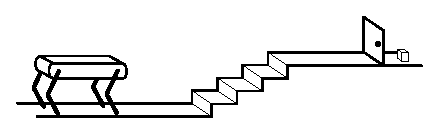
\includegraphics[width=0.9\columnwidth]{task.eps}
    \vspace{1em}
\caption{The \emph{fetching} task considered in the design case study (\T{3}). 
In this scenario, the robot must execute multiple complex behaviors:
(1) locomote on flat ground; 
(2) climb stairs; 
(3) open a cabinet door; 
and 
(4) pick up an object.
}
    \label{fig:task}
\end{figure}

For this case study we choose to focus on a \emph{fetching} task, as shown in Figure~\ref{fig:task}. For concreteness we will define the case study in term of a home assistance robot that you might command to retrieve an object from a cabinet upstairs, though the same capabilities are of use to many other applications domains such as urban search and rescue or explosive ordnance disposal.
We break this task down into four behaviors: 1) locomotion on flat ground, 2) stairclimbing, 3) operating cabinets and drawers, and 4) picking up an object. Defining good reduced order models for these behaviors is essential to the proposed research. 
{\bf The key challenge in this subtask (\T{3.1}) is to define the reduced order models that will serve as the basis for this case study}.

A wide range of animals would be capable of accomplishing this task, though they would use different strategies based on their body size and design. Humans would rely on two appendages exclusively for walking, and a separate two appendages with dexterous end effectors for the manipulation tasks. A monkey might use some combination of all four appendages for each. A dog might use all four legs for locomotion, and switch to using their mouth to pick up and carry the object. A bird would fly up the stairwell to the cabinet and then use its beak or feet to pry it open and retrieve the object. Unconstrained by biological forms, we can imagine an even wider range of engineered systems as well that are all capable of accomplishing these tasks. A robot could use legs, tracks, or compound wheels to traverse the stairs. The object could be retrieved with a gripper or suction cup as an end effector. 

\begin{figure}[b]
    \vspace{.5em}
    \centering
    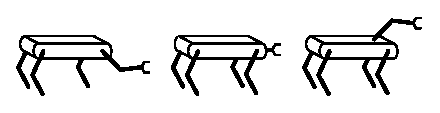
\includegraphics[width=0.9\columnwidth]{bodies.eps}
    \vspace{.5em}
\caption{Three body types will be considered, all starting from a common quadrupedal base and adding a gripper on (left) a foot, (center) the body (as a ``mouth''), or (right) an additional arm. In each case, the design will consider the lengths of all limbs, the actuator selection for the gripper, and the design of the fingers. }
    \label{fig:bodies}
\end{figure}

In this case study, we will consider three candidate robot bodies, shown in Figure~\ref{fig:bodies}, all based on a quadrupedal design that add manipulation capabilities in the form of a gripper attached to either 1) a foot, 2) the body (as a ``mouth''), or 3) to the end of an additional appendage as an ``arm''.  The design of the robot will consider the lengths of the various limb segments, the actuator selection in the gripper, and the design of the fingers.  With many candidate robotic designs and multiple behaviors (resulting in multiple reduced-order models), the need for formal synthesis methods of \T{1} for generating the morphological reductions is clear.  {\bf The key challenge in this subtask (\T{3.2}) is to generate the set of morphoogical reductions by using the methods derived in \T{1}.}

This particular collection of candidate morphologies is also designed to enable low cost and rapid evaluation by all being based on a single quadrupedal robot core, which will be the Ghost Robotics Minitaur \cite{Kenneally2016-ml}. The PIs collectively own three of these platforms, and they are easy to customize by varying the leg lengths and adding additional end effectors. This robot also is an interesting case study in the need for multibehavioral design. While it was designed with walking, running, and jumping in mind \cite{Kenneally2015-yj,Kenneally2016-ml}, it turns out to be ill-suited to stairclimbing \cite{topping2017quasi,tr:ren2018riss}. While it can climb stairs, the spacing between the hips is such that normal, human-sized stairs are challenging to climb in the usual manor, and so a jumping climb must be used instead. Thus even designing a robot for locomotion on flat ground and stairwells provides interesting tradeoffs that we hope to address with this case study. 

As shown in Figure~\ref{fig:tasks}, these behaviors naturally introduce many tradeoffs in the design of the robot. Locomotion tasks benefit from having low total mass, and in particular low distal mass, while manipulation tasks would prefer to have large, powerful end effectors available at the robots farthest reach. It can be difficult to reason about these tradeoffs, because the performance on each behavior may be sensitive to most if not all of the robot's body parameters. However, the dimensionality of the tradespace, and ultimately the Pareto optimal solution set, is much lower and can allow the designer to more directly consider tradeoffs at the behavior level and not consider every morphological parameter independently. {\bf The key challenge in this subtask (\T{3.3}) is to characterize the design tradespace and explore the Pareto optimal designs (using the methods from \T{2}) to generate designs that are successful on all of the desired behaviors. These designs will then be built and tested on the robot hardware. }


\begin{figure}
    \centering
    \begin{tikzpicture}[node distance=4cm, auto]
     %nodes
     \node (walk) {\Large Walking};
     \node[below=2cm of walk] (stair) {\Large Stair Climbing};
     \node[right=of walk] (open) {\Large Open Cabinet};
     \node[below=2cm of open] (obj) {\Large Pick Up Object};
     
     
    \draw[<->, very thick] (walk.east) to [out=20,in=160] (open.west);
    \draw[<->, very thick] (walk.south) to [out=-110,in=110] (stair.north);
    \draw[<->, very thick] (stair.east) to [out=-20,in=-160] (obj.west);
    \draw[<->, very thick] (open.south) to [out=-70,in=70] (obj.north);
    \end{tikzpicture}
    \caption{Figure showing the four behaviors indicating tradeoffs between each, e.g. walking wants low mass but open cabinet wants big gripper, stair climbing wants longer legs to step over things while walking wants shorter legs to minimize cost, pick up object wants gripper on long arm, open cabinet would prefer extra strength from mouth option that can pull with all legs}
    \label{fig:my_label}
\end{figure}

\begin{figure}
    \centering
    \includegraphics{arrows.pdf}
    \caption{Alternate Figure showing the four behaviors indicating tradeoffs between each, e.g. walking wants low mass but open cabinet wants big gripper, stair climbing wants longer legs to step over things while walking wants shorter legs to minimize cost, pick up object wants gripper on long arm, open cabinet would prefer extra strength from mouth option that can pull with all legs}
    \label{fig:my_label}
\end{figure}

How to best manage these tradeoffs among the possible Pareto optimal set is surely an application-specific question. Some scenarios may not require stairclimbing, or may have heavier objects to retrieve, changing the relative importance of the various performance metrics. A key advantage of the analysis proposed in \T{1} and the design synthesis of \T{2} is the ability to quickly customize the design to meet the current need. A designer can either match the robot exactly to their problem, or explore the sensitivity of the chosen design to variations in the design tradeoffs. As part of this case study, we will explore this idea of customizability by varying the parameters of the scenario. {\bf The key challenge in this subtask (\T{3.4}) is to test how these methods lead to more easily customized designs, and evaluate the benefit of that customization on the task performance.}


\paragraph{Notes from aaron/tom call:}
\begin{itemize}
    \item Behaviors will be climbing stairs, locomotion on flat ground, opening a drawer/cabinet, and picking up an object inside
    \item There will be a few versions of the scenario, where we change the relative importance (e.g. longer flat walking, or heavier object) and can quickly customize the design to a scenario
    \item Will consider 3 basic bodies all based on minitaur. One adds a gripper at the foot, one adds a gripper at the "mouth" (body), and one adds an extra minitaur leg on top as an arm with a gripper at the end. Parameters include link lengths of the legs/arms, actuator selection for the gripper, mass and size of added gripper.
    \item Comparison will be to other design methods, not to other designs. We are not saying that spot mini or any other robot is not capable of doing these, but rather that if you wanted to design such a robot this is how you could do it
    \item Tasks: 3.1 develop reduced order and full robot models to be used, 3.2 apply T1 and T2 to do the anchoring and design, 3.3 adjust the specs and see the customizability
    \item Figure: have a cartoon or posed photo of minitaur for each of the 4 behaviors, with arrows between different behaviors showing the tradeoff. Between stairclimbing and walking, the stairclimbing wants longer legs to step over things but the walking wants shorter legs to reduce the torque requirement. Between walking and object manip the walking wants to minimize mass and the manip wants the biggest and strongest gripper available, between manip and climbing the climbing wants smaller feet to avoid collision while the manip wants the dexterity that comes from having the gripper at the end of the leg while cabinet/drawer would prefer the mouth where you can use the strenght of all legs and not be limited to one leg, etc.
\end{itemize}


\sect{Intellectual Merit}
%The Project Description must contain, as a separate section within the narrative, a section labeled "Intellectual Merit". The Project Description should provide a clear statement of the work to be undertaken and must include the objectives for the period of the proposed work and expected significance; the relationship of this work to the present state of knowledge in the field, as well as to work in progress by the PI under other support.

%The Project Description should outline the general plan of work, including the broad design of activities to be undertaken, and, where appropriate, provide a clear description of experimental methods and procedures. Proposers should address what they want to do, why they want to do it, how they plan to do it, how they will know if they succeed, and what benefits could accrue if the project is successful. The project activities may be based on previously established and/or innovative methods and approaches, but in either case must be well justified. These issues apply to both the technical aspects of the proposal and the way in which the project may make broader contributions.


This project will develop tools for analysis and design that will enable researchers to build more capable robotic systems. In particular, this \emph{design-for-multibehavioral robots} paradigm has the potential to lead to systems that are more than just the sum of their parts.  

In addition to the specific modeling and design algorithms, this project will advance our understanding of the structure of how behaviors relate to both their embodied robot designs, as well as to other behaviors. By providing structure to these form/function relationships, we hope to expose the underlying tradeoffs and limitations that a robot design entails. 

Finally, the particular case study of a fetching robot in \T{3} entails a particular collection of desired behaviors that are desirable for many long-dreamed robotic applications. Home assistance, either for domestic help in the spirit of Rosie in the Jetsons or as an elder assistant to help people age in place, has been an increasing focus of robotics researchers \cite{something}. But the same behaviors of locomotion over clutter, operating doors and drawers, and fine motor skills are also necessary in explosive ordnance disposal (EOD), teleoperation in hazardous environments such as after a nuclear disaster, or scientific sampling in remote locations. 



\sect{Broader Impacts}
%The Project Description also must contain, as a separate section within the narrative, a section labeled "Broader Impacts". This section should provide a discussion of the broader impacts of the proposed activities. Broader impacts may be accomplished through the research itself, through the activities that are directly related to specific research projects, or through activities that are supported by, but are complementary to the project. NSF values the advancement of scientific knowledge and activities that contribute to the achievement of societally relevant outcomes. Such outcomes include, but are not limited to: full participation of women, persons with disabilities, and underrepresented minorities in science, technology, engineering, and mathematics (STEM); improved STEM education and educator development at any level; increased public scientific literacy and public engagement with science and technology; improved well-being of individuals in society; development of a diverse, globally competitive STEM workforce; increased partnerships between academia, industry, and others; improved national security; increased economic competitiveness of the US; and enhanced infrastructure for research and education.

The analysis and design methods developed in this proposal will enable  multibehavioral robots that can work better in human environments. 
As we strive for robots that can work outside of a factory or warehouse setting, we can no longer simply combine many single behavior mechanisms (e.g.\ conveyor belts, pick and place arms, spot welding robots, etc) to complete the desired tasks. We are particularly interested in enabling better home assistance robots, such as the fetching robot presented here. In order to work well in a home environment a robot must use a wide variety of behaviors to navigate over messy floors, climb up stairs, operate drawers and cabinets, etc.

One of the goals of NRI2.0 is to lower the barriers to entry into robotics research. This project will make it easier to design complex robots that can to do a variety of behaviors, which will help open up robotics to a wider range of researchers around the world. By no longer being constrained to single-behavior robots or combining off-the-shelf designs, these researchers can expand the range of what is possible with robotics. 

Creating more capable robots, such as the fetching robot from \T{3}, will provide a more exciting and engaging example for outreach. The PIs all have a long history of STEM outreach and strive to inspire young students to pursue a career that will positively impact the world. To enhance these efforts, we plan to integrate the results of this project in two continuing programs. First, PI Johnson runs a workshop as part of the ``Engineering\@CMU'' program where a class of high school students from Pittsburgh Public Schools comes to campus to learn about engineering. The idea of design tradeoffs is a fundamental one in engineering, and we will build a curriculum using this platform that lets the students see the consequences of these tradeoffs in action. The second program, PI Burden ... (And/or Co-PI Libby)

Finally, we plan to integrate the results of this project into the curriculum of the PI's courses at the collegiate level. Specifically, PI Johnson plans to integrate the results of this project into a new unit for his class ``Robot Dynamics and Analysis''. This new unit will cover design and analysis techniques that use lower-dimensional dynamical models and how to relate those back to the full robot dynamics. PI Burden ... (And/or Co-PI Libby)


\sect{Results from Prior NSF Support}
\begin{comment}
The purpose of this section is to assist reviewers in assessing the quality of prior work conducted with prior or current NSF funding. If any PI or co-PI identified on the proposal has received prior NSF support including:
* an award with an end date in the past five years; or
* any current funding, including any no cost extensions,

information on the award is required for each PI and co-PI, regardless of whether the support was directly related to the proposal or not. In cases where the PI or any co-PI has received more than one award (excluding amendments to existing awards), they need only report on the one award that is most closely related to the proposal. Support means salary support, as well as any other funding awarded by NSF, including research, Graduate Research Fellowship, Major Research Instrumentation, conference, equipment, travel, and center awards, etc.

The following information must be provided:

(a)	the NSF award number, amount and period of support;

(b)	the title of the project;

(c)	a summary of the results of the completed work, including accomplishments, supported by the award. The results must be separately described under two distinct headings: Intellectual Merit and Broader Impacts;

(d)	a listing of the publications resulting from the NSF award (a complete bibliographic citation for each publication must be provided either in this section or in the References Cited section of the proposal); if none, state “No publications were produced under this award.”

(e)	evidence of research products and their availability, including, but not limited to: data, publications, samples, physical collections, software, and models, as described in any Data Management Plan; and

(f)	if the proposal is for renewed support, a description of the relation of the completed work to the proposed work.

If the project was recently awarded and therefore no new results exist, describe the major goals and broader impacts of the project. Note that the proposal may contain up to five pages to describe the results. Results may be summarized in fewer than five pages, which would give the balance of the 15 pages for the Project Description
\end{comment}

\noindent\textbf{Johnson}
\emph{RI: Small: Smarter Hands with Direct-Drive Actuation} 
(\#RI--1813920) PI: Mason, Co-PI: Johnson, \$499,297 (2018/08/15--2021/07/31) \\
{\it Intellectual Merit:} This project explores basic principles in the design of robotic manipulation focused on transparency to the environment. The project is developing a set of models that view the hand as a set of information channels, and using the insights from
those models to build direct-drive hands that efficiently transmit information, encoded as motion and force, between task
and robot. The project is also developing intelligent behaviors, controls, and planning algorithms to exploit
the information. Performance will be evaluated on sample tasks: touch localization and manipulation in
clutter; high speed grasping; picking up thin objects; fine motor games like Jenga; and industrial applications
including small part assembly and flexible cable insertion. Results demonstrating these design principles and concept reactive behaviors are presented in \cite{paper:bhatia-direct-2019}.\\
{\it Broader Impacts:}  This project will expand the effectiveness of robotic manipulators in new applications,
primarily those where sensitivity of touch, fast finger motion, and compliant manipulation in
unstructured environments is required. Direct-drive hands are well suited to research in human robot interaction. The ability to sense external
forces and the mechanical transparency to external impacts complements current work in collaborative robot
arms. The direct-drive hand can also exhibit a range of compliant behaviors which is important in the study
of human-robot handovers.
The simplicity of direct-drive actuation means that this technology can be made readily available to
the robotic manipulation community. The low mass is suited to lighter less expensive arms, well-suited to
educational settings and in developing countries where price is a limiting factor.

\noindent\textbf{Burden}
\emph{CRII: CPS: Provably-safe interventions for Human-Cyber-Physical Systems (HCPS)} 
(\#CNS--1565529) PI: Burden, \$182,002 (2016/04/01--2018/03/31) \\
{\it Intellectual Merit:}  performance guarantees when humans interact in closed loop with autonomy.
Published theoretical approach~\cite{Robinson2016-qh}, review~\cite{Nothwang2016-jj}, experimental validation~\cite{Roth2017-jp, Yamagami2018-nm}.
{\it Broader Impacts:}  safe teleoperated robots provide emergency response services in urban areas.

\noindent\textbf{Libby} \emph{No prior NSF funding to report.}



\pagebreak
\setcounter{page}{1}

%\sects{Supplementary Documents}


\sects{Collaboration Plan}

% A Collaboration Plan is REQUIRED for projects with more than one investigator, even if the investigators are from the same institution. The Collaboration Plan must be submitted as a Supplementary Document and cannot exceed two pages. 
% PROPOSALS THAT REQUIRE A COLLABORATION PLAN, BUT DO NOT SUBMIT ONE, WILL BE RETURNED WITHOUT REVIEW. 
% The Collaboration Plan must be labeled "Collaboration Plan" and must provide a thoughtful, strong justification for the team of researchers. 

% THE COLLABORATION PLAN MUST INCLUDE: 

% 1) the specific roles of the collaborating PIs, co-PIs, other Senior Personnel and paid consultants at all organizations involved; 
% 2) how the project will be managed among participants, especially across institutions and disciplines, with a description of how the researchers will work together collaboratively and effectively; 


\paragraph{Specific roles of the collaborating PIs and project management}
%The technical objectives of this proposal will be achieved by integrating and advancing state-of-the-art techniques in several different domains including: dynamical systems and control theory; hybrid systems theory; reinforcement learning; multi-agent systems and game theory.

%The team brings complementary expertise, as described above, and is well-positioned to successfully complete the proposed work. 

Expertise from the three PIs will be leveraged to address research challenges in the three technical threads discussed in the Technical Approach.
For each of the three testbeds discussed in Section 2, two PIs will collaboratively lead evaluation efforts. 
The first PI listed for each testbed will be hold primary responsibility for coordinating implementation logistics, but both PIs listed will contribute relevant domain knowledge and technical expertise. 

The PIs and the graduate students involved in this project will participate in biweekly meetings via videoconference to provide updates on project status. %The entire project team will coordinate to publish and disseminate the research results. 
%PI Coogan will be responsible for reporting research results to NSF. 
At least once per year, the three PIs will meet in person to discuss research progress. 
Moreover, travel funds have been budgeted to allow students from Carnegie Mellon University to visit the University of Washington during the summer, and vice versa.  
A wiki website with a public and private portal will be created to manage and share research progress. 
Publications and research results will be shared through the public portal. 
The private portal will allow easy sharing of ideas and progress among team members and with the broader robotics research community. 



% 3) identification of the specific coordination mechanisms that will enable cross-institution and/or cross-discipline scientific integration (e.g., workshops, graduate student exchange, project meetings at conferences, use of videoconferencing and other communication tools, software repositories, etc.); 
% 4) SPECIFIC REFERENCES TO THE BUDGET LINE ITEMS THAT SUPPORT THESE COORDINATION MECHANISMS


\paragraph{Identification of specific coordination mechanisms}
To facilitate the yearly meetings between PIs, the proposed budget includes an extra day in Washington DC so that the PIs can meet after the NRI PI Meeting. 
Moreover, the PIs will collaborate and coordinate on the Broader Impacts activities described above, including: 
developing and teaching the graduate-level seminar on robot design in year 2; 
and developing and piloting the undergraduate-level curriculum in year 3.

%---------------------------------------------------------------------------
\pagebreak
\setcounter{page}{1}

\sects{Data management plan}

% Plans for data management and sharing of the products of research, including preservation, documentation, and sharing of data, samples, physical collections, curriculum materials and other related research and education products should be described in the Special Information and Supplementary Documentation section of the proposal (see Chapter II.C.2.j for additional instructions for preparation of this section).
% 
% Plans for data management and sharing of the products of research. Proposals must include a document of no more than two pages uploaded under "Data Management Plan" in the supplementary documentation section of FastLane. This supplementary document should describe how the proposal will conform to NSF policy on the dissemination and sharing of research results (see Chapter XI.D.4), and may include:
% 
% the types of data, samples, physical collections, software, curriculum materials, and other materials to be produced in the course of the project;
% 
% the standards to be used for data and metadata format and content (where existing standards are absent or deemed inadequate, this should be documented along with any proposed solutions or remedies);
% 
% policies for access and sharing including provisions for appropriate protection of privacy, confidentiality, security, intellectual property, or other rights or requirements;
% 
% policies and provisions for re-use, re-distribution, and the production of derivatives; and
% 
% plans for archiving data, samples, and other research products, and for preservation of access to them.
% Data management requirements and plans specific to the Directorate, Office, Division, Program, or other NSF unit, relevant to a proposal are available at: http://www.nsf.gov/bfa/dias/policy/dmp.jsp. If guidance specific to the program is not available, then the requirements established in this section apply.
% 
% Simultaneously submitted collaborative proposals and proposals that include subawards are a single unified project and should include only one supplemental combined Data Management Plan, regardless of the number of non-lead collaborative proposals or subawards included. In such collaborative proposals, the data management plan should discuss the relevant data issues in the context of the collaboration.
% 
% A valid Data Management Plan may include only the statement that no detailed plan is needed, as long as the statement is accompanied by a clear justification. Proposers who feel that the plan cannot fit within the limit of two pages may use part of the 15-page Project Description for additional data management information. Proposers are advised that the Data Management Plan must not be used to circumvent the 15-page Project Description limitation. The Data Management Plan will be reviewed as an integral part of the proposal, considered under Intellectual Merit or Broader Impacts or both, as appropriate for the scientific community of relevance.


% 1. the types of data, samples, physical collections, software, curriculum materials, and other materials to be produced in the course of the project;
\subsection*{1. Types of data, software, and outreach materials}

\paragraph{telelocomotion testbed:}
to support this proposal's technical objectives, we will develop a \emph{telelocomotion testbed} based on the Robot Operating System ({\tt\ROS})~\citesf{QuigleyConley2009}.
This testbed will consist of a graphical interface based on the Robot Visualization ({\tt rviz}) environment bundled with {\tt\ROS} together with underlying codes that interface with haptic input devices, virtual/augmented reality headsets, and robots (both simulated and physical).


\paragraph{Software:}
in the parlance of {\tt\ROS}, we will develop {\tt{\ROS} nodes} that can be flexibly redeployed by other researchers for
haptic interaction,
virtual/augmented reality,
and
telerobotics.

\paragraph{Data and metadata:}
experimental data will consist of
(i) metadata describing the experimental protocol in effect
and
(ii) time series of:
forces applied to and received from the human operator via haptic devices;
states (e.g. positions and velocities of joint segments) of the teleoperated robot (whether simulated or physical).
Our guiding principle is to record all and only the data needed to reproduce every experiment and analysis conducted in support of the proposed research.

\paragraph{Outreach materials:}
a modified version of the telerobotic testbed software will be developed and employed for {\KTW} {\STEM} outreach as described in the Broader Impacts section of the Project Description of this proposal.

% 2. the standards to be used for data and metadata format and content (where existing standards are absent or deemed inadequate, this should be documented along with any proposed solutions or remedies);
\subsection*{2. Standards for data and metadata}

\paragraph{Raw data and metadata:}
will be recorded in a {\tt{\ROS} bag}, which is an open source data format developed for the {\tt{\ROS}} software platform.
This data format is stable and ensured to be both backward and forward compatible with different versions of {\tt{\ROS}}.

\paragraph{Analyzed data and metadata:}
will be stored in a human--readable {\tt\JSON} file format that is easily parsed by modern scripting and programming languages (e.g. {\tt\Python}).

\subsection*{3., 4., 5. Policies for access, re--use, and archiving}

% 3. policies for access and sharing including provisions for appropriate protection of privacy, confidentiality, security, intellectual property, or other rights or requirements;
%\subsection*{3. Policies for access and sharing}
\paragraph{Access to data:}
de--identified data, as well as algorithms, will be posted and made publicly available after the supporting publications have been accepted in a peer--reviewed journal.

% 4. policies and provisions for re-use, re-distribution, and the production of derivatives; and
%\subsection*{4. Policies and provisions for re--use, re--distribution, and archiving}
\paragraph{Re--use of data or software:}
individuals using these products will be asked to cite the corresponding publication that contains the research they are using or building upon.
Data not used in publications will be available upon request after a discussion between the PIs and the requesting group to establish an agreement for data use, publication, and distribution.
Testbed software will be versioned and released freely in public repositories on a popular free and open--source software hosting website, GitHub\footnote{\url{http://github.com}}.

% 5. plans for archiving data, samples, and other research products, and for preservation of access to them.
%\subsection*{5. Plans for archiving data and other research products}

\paragraph{Archiving data:}
Generated data will initially be stored locally on the data collection workstation. This data will be uploaded on a daily basis to a central data archive server that conducts periodic offsite backups.
Long--term data retention will be ensured through posting to GitHub.

%Plans for transition or termination of data collection
%In the event that data collection is terminated, we will continue to maintain archived data for a minimum of 5 years after termination. During this period, long-term data storage will be examined, including repositories. If the PI leaves the institution, with the support of the Institutional Review Board for Human Subjects Research, coded data will be transferred to a new institution, if research will be continued. Otherwise, data will be archived for 5 years after the transition.


%---------------------------------------------------------------------------
\pagebreak
\setcounter{page}{1}

\sects{Postdoctoral Researcher Mentoring Plan}
%In no more than one page, the mentoring plan must describe the mentoring that will be provided to all postdoctoral researchers supported by the project, regardless of whether they reside at the submitting organization, any subrecipient organization, or at any organization participating in a simultaneously submitted collaborative project.
%Mentoring activities provided to postdoctoral researchers supported on the project will be evaluated under the Broader Impacts review criterion.
%Examples of mentoring activities include, but are not limited to:
%career counseling;
%training in preparation of grant proposals,
%publications and presentations;
%guidance on ways to improve teaching and mentoring skills;
%guidance on how to effectively collaborate with researchers from diverse backgrounds and disciplinary areas;
%training in responsible professional practices.


% %Instructions
% %
% %Postdoctoral Researcher Mentoring Plan. Each proposal28 that requests funding 
% to support Postdoctoral researchers must include, as a supplementary document, a 
% description of the mentoring activities that will be provided for such 
% individuals. In no more than one page, the mentoring plan must describe the 
% mentoring that will be provided to all Postdoctoral researchers supported by the 
% project, irrespective of whether they reside at the submitting organization, any 
% subawardee organization, or at any organization participating in a 
% simultaneously submitted collaborative project. Proposers are advised that the 
% mentoring plan may not be used to circumvent the 15-page project description 
% limitation. See GPG Chapter II.D.4 for additional information on collaborative 
% proposals
% %
% %Examples of mentoring activities include, but are not limited to: career 
% counseling; training in preparation of grant proposals, publications and 
% presentations; guidance on ways to improve teaching and mentoring skills; 
% guidance on how to effectively collaborate with researchers from diverse 
% backgrounds and disciplinary areas; and training in responsible professional 
% practices. The proposed mentoring activities will be evaluated as part of the 
% merit review process under the Foundation's broader impacts merit review 
% criterion. Proposals that include funding to support Postdoctoral researchers, 
% and, do not include the requisite mentoring plan will be returned without review 
% (see GPG Chapter IV.B.)


This project provides partial support for one Postdoc in each year of the project, expected to be co-PI Dr.\ Thomas Libby. 
Dr.\ Libby is currently a member of PI Burden's laboratory, The University of Washington BioRobotics Laboratory ({\BRL}),
and plans to remain at {\UW} for 
approximately three more years. 
Dr. Libby possesses expertise in bio-inspired design; he will direct execution of the \emph{case study} and experimental work at UW through collaboration with co-PI Burden.  
He has demonstrated
an extraordinary level of productivity 
in {\BRL}.
The components of the comprehensive mentoring plan 
for this Postdoc is described below.

\paragraph{Weekly meetings with the PIs:} The Postdoc will meet on a 
weekly basis with co-PIs Burden and Johnson (who will attend virtually) for at least one hour to discuss both technical and professional 
development issues. 
The Postdoc will be included in the
intellectual leadership of the research, will be encouraged to
develop their own unique line(s) of research, and to produce
first--author publications of that work. 

\paragraph{Weekly Lab meetings:} 
The University of Washington BioRobotics Lab consists of about 20 graduate and 
10 undergraduate researchers, and two Postdocs, under the direct supervision of
three faculty members, Profs. Sam Burden, Blake Hannaford, and Howard Chizeck. 
Thus the weekly lab meetings of the BRL will 
expose the Postdoc to a variety of leadership and scholarship styles, and 
provide rich opportunities for collaboration.  
The Postdoc will be given the task of soliciting outside speakers and scientific topics for this weekly meeting series.

\paragraph{Teaching opportunities:}  From time to time, Postdocs and senior 
Ph.D. students in the ECE Department at the University of Washington serve as the instructor of record, typically for established graduate courses in their 
areas of specialization.  This is a very strong career development opportunity 
for any student or Postdoc considering a future faculty career.   If sufficient 
time is not available or a suitable course is not open, the Postdoc will be 
encouraged to give substitute lectures, design and help grade an exam, or participate in other short-term  projects to provide them with teaching experience. 
Furthermore, a Postdoc in the BRL is expected to mentor one or more beginning graduate and 
undergraduate researchers as they collaborate on projects. 

\paragraph{Networking opportunities:}  The Postdoc will have two chief networking opportunities.  
First will be attending and helping to organize monthly meetings, seminars, and colloquia associated with interdisciplinary institutes and groups on {\UW}'s campus; this will expose the Postdoc to a diverse group of scientists and engineers working across campus the broader Seattle tech community, as well as visitors to said campus and community.
 Secondly, the research conducted in this project will be published in 
conference publications which will enable the Postdoc to travel to leading 
conferences. 

\paragraph{Proposal writing:} Postdocs in the UW BioRobotics laboratory are recruited to 
assist with the development of proposals related to the Postdocs' interests, as 
well as to assist in completion of required reports, invention disclosures, etc. 
This educates the Postdoc in fundraising and administrative skills 
necessary to manage a successful lab, whether in academia or industry.  

\paragraph{University Level Resources:}
The University of Washington has an official Postdoc Career Development program 
with an active series of seminars and events%
\footnote{\url{http://www.grad.uw.edu/profdev/Postdoc.shtml}}%
, which the Postdoc will be encouraged to participate in.


\pagebreak


% DARPA Q's (Heilmeier catechism) -- answer first 4 on first page
% 1. What are you trying to do? Articulate your objectives using absolutely no jargon.
% 2. How is it done today, and what are the limits of current practice?
% 3. What's new in your approach and why do you think it will be successful?
% 4. Who cares? If you're successful, what difference will it make?
% --
% 5. What are the risks and the payoffs?
% 6. How much will it cost? How long will it take?
% 7. What are the midterm and final "exams" to check for success?

\subsects{Innovation and Motivation}

%A robot's mechanical design \AJ{Are we only considering mechanical design and not controller/sensor/software design?} often limits its behavioral repertoire.
%For instance, industrial manipulators that are effective at pick-and-place can only help with tasks that lie within reach.
%Similarly, mobile robots designed to traverse air, ground, or water have limited ability to grab objects in their environment.
A robot's behavioral repertoire is ultimately limited by its mechanical design or \emph{morphology}: the shape and composition of its body parts as well as the capability of actuators and sensors. 
% if it's a plural robot above, it should be plural below, and vice-versa
In turn, this repertoire determines the robot's ability to perform complex tasks. A wheeled mobile manipulator might be good at pick-and-place, but be unable to climb a stairwell. A small legged robot might crawl under a chair, but be unable to jump onto a table. 
%A robot capable of reaching every space in a dwelling and manipulating every object would be prohibitively expensive (if even possible), so practicable machines face design tradeoffs that shape the behaviors they can perform.
%\SB[inline]{I'm totally onboard up until here, but the transition to the next sentence was rough for me.  I think the last sentence above isn't quite what we want, because it actually makes me think that design for multibehaviorality will be too hard, or the resulting designs will be so compromised as to be impractical / unusable.}
%\AJ{I commented out sam's note and took a stab at fixing it:}
Robots that can perform all of these behaviors are challenging to design since the ensemble of behaviors may have conflicting requirements that are not readily apparent due to the complexity of the dynamic relationship between design and behavior.
In this work, we will establish and apply a \emph{design methodology for multibehaviorality} that enables creation of multibehavioral robots by systematically negotiating performance tradeoffs in a complex design space.
% Enabling robots to perform complex, dynamic tasks therefore requires that is,
% a design methodology that simplifies the problem of considering multiple behavioral objectives.
%\dots\SB{I think we should have a succinct definition here}
%the desired behavioral repertoire must be taken into account when creating a robot's morphology 
%(lengths, masses, number and arrangement of actuators, etc).
%\SB{what all should be / do we want to include in morphology?}

For concreteness, consider a \emph{fetching} task wherein
a home robot assistant may retrieve medicine from a cabinet or bag, or
a field robot may retrieve a soil sample from under a rock.
These tasks could be accomplished by either large (e.g. humanoid) or small (cat or even rat sized) robots.
%\TL{I bet most readers are thinking of a large humanoid robot at this point -- I'm trying to encourage them to think smaller}
At any scale, the robot must employ a sequence of \emph{behaviors} including, e.g.:
locomoting over stairs, furniture, or grass; moving obstacles in its path;
and
manipulating objects buried in cabinets, bags, or underground.
Although challenges remain in perception, planning, and control for each of these behaviors,
we claim that morphology constrains the behavioral repertoire of existing robots as much or more than algorithmic limitations.
As evidence of this claim, note that there exist robots that competently perform each of the behaviors listed above, yet there is no robot proficient at every behavior in such a diverse repertoire.


If successful, this project will produce analytical and computational tools that enable the systematic investigation of tradeoffs that naturally arise when designing for multibehaviorality.
Continuing with the fetching example, clear tradeoffs exist between the manipulation 
behaviors, which benefit from more dexterous (but heavier) hands, and the locomotion behaviors, which benefit from lighter limbs. 
To address the challenge of comparing and selecting candidate morphologies for a multibehavioral design problem, we will leverage predictive dynamical models at multiple levels of abstraction.
Our approach will provide insights into qualitative aspects of reduced-order representations of behavior without losing a quantitative connection to the details of morphology that are the actual targets for design. 
% A key challenge in robot design is identifying and exploiting the freedom available to the designer:
% selection of body shape %(scale, number and arrangement of limbs) 
% and components %(materials, sensors, actuators, computers) 
% to meet performance specifications required by a behavior. 
The paradigm 
we propose will simultaneously synthesize the suite of desired behaviors and the mechanical design: a \emph{co-design} of the platform and multiple behaviors.
This approach will reveal relationships between morphology and performance, exposing tradeoffs between behaviors and fitness comparisons between robot bodies.

\subsects{Approach and Preliminary Results}

%\TL{I think we decided to fold state of the art into this section, right? I've done so, but feel free to countermand}
\paragraph{T1 Multi-scale modeling} 
Reduced-order models of locomotion have provided valuable insights into the principles underlying stability and efficiency of periodic behaviors including walking~\citesf{McGeer1990-zb, Collins2005-sc, Srinivasan2005-hz}, running~\citesf{Blickhan1993-sr, Seipel2004-ag}, %, Srinivasan2005-hz
%turning~\citesf{Jindrich1999-sb, Proctor2008-ks}, 
jumping~\citesf{Aguilar2012-vn, Johnson2013-rt,  Haldane2016-qq}, %Burden2015-ru, Libby2012-xl,
and climbing~\citesf{Clark2007-ds, Goldman2006-cf}.
% In recent work, we proposed a multi-scale modeling framework for exactly embedding reduced-order models like these 
% in higher-fidelity counterparts 
% (that include detailed design parameterizations)~\citesf{Burden2015-ru}, 
% providing insight into the role of morphology in inertial reorientation behaviors~\citesf{paper:libby_tail_2016}.
% \TL{Need to compare to surrogate model approach here; I guess the main difference is that we start with a first-principles mechanical system as our template, whereas surrogates are data-driven.}
% We propose to extend these preliminary results to formalize approximate embeddings between models at multiple levels of abstraction and to create algorithms that derive these embeddings directly from experimental data.
% \TL{We say "multiple" several times; would it be easier to understand if we just lay out simple/complex (i.e. two levels)? Any benefit to hedging on number like this?}
% These advances will reveal form/function relationships that detail how morphology shapes performance, e.g. how
% the choice of leg length or motor power is constrained by the performance requirements of a behavior. 
% These problems will typically be underdetermined, resulting in unresolved freedom (a \emph{morphological nullspace}, e.g.\ all combinations of leg length and motor power that enable locomotion at a given speed). 
% Our objective is to expose this freedom to the designer explicitly, aiding both optimization-based and iterative design approaches and setting the stage for multibehavioral design. 
% \AJ{Should the phrase pareto set appear here? Or later?}
% \SB{If we say Pareto, I think we should say it in T2, not T1}
% \TL{There's no reason a single behavior couldn't have multiple objectives to trade off (our tails example had reorientation angle and duration). But I think it's easier to work into T2.}
The mechanistic understanding provided by these simple models has been exploited for analysis~\citesf{full1999templates} and design~\citesf{hubicki2016atrias} by using them to predict the motion of a more morphologically-representative model performing the behavior of interest. 
This implies the existence of a map between the design space of a robot (e.g. parametrization of its representative model~\citesf{Burden2015-ru}) and the parameters of its reduced-order representation.  Our recent work explicated and exploited this parameter reduction %\emph{Morphological Reduction}
to design morphology for inertial reorientation behaviors~\citesf{paper:libby_tail_2016}. 
In contrast to surrogate modeling~\citesf{forrester2008engineering}, where reduced-order models are data-driven, our approach leverages the mechanistic insight encoded in the simple model to simplify the design space.
We propose to extend these preliminary results to formalize approximate embeddings between models at multiple levels of abstraction.
Whereas an ideal optimizer could in theory fully exploit the mechanics of a morphology to maximize performance (potentially finding solutions unforeseen by the designer), our approach restricts behavior to possibilities predicted by the reduced model. The payoff is a dramatic reduction of complexity, enabling insight into the role of morphology and robustness to the challenges of hardware implementation of model-based designs.

\paragraph{T2 Multibehavioral design}  
% Traditional design algorithms extremize single or multiple objective 
% functions using local descent or global search~\citesf{marler2004survey,deb2014multi}; the challenge 
% for multibehavioral design is
% simultaneous satisfaction of competing behavioral constraints without resulting in an intractable problem.
% Design of complex systems like automobiles is often decomposed into a hierarchy of subproblems wherein optimization of detailed models is tractable; 
% for instance,
% target cascading~\citesf{kim2003target,michalek2005linking} and cooperative multi-optimization~\cite{tappeta1997multiobjective} work to ensure that the high-level system is feasible and consistent. However, these methods rely on a single, well-defined objective function to evaluate task performance. 
% No principled methods exist to specify this cost function for a multibehavior robot; 
% na{\"{i}}ve weighting of behaviors could cripple task performance, as the optimizer maximizes performance in some behaviors at the cost of others.
% These observations motivate our focus on deriving analytical and computational tools to characterize \emph{constraints} and \emph{tradespaces} imposed by multibehavioral design. 
% \SB{What's a tradespace?}
% \AJ{This should connect to the morphological nullspace we define above, or that needs to be changed}

Adding behaviors to a robot's repertoire increases the number of design objectives and, thus, design tradeoffs. 
A common approach to navigating these tradeoffs is multi-objective optimization~\citesf{marler2004survey,deb2014multi}. 
If preferences about the importance of each behavior can be quantified, then principles of optimality determine the preferred design. 
However, these preferences are notoriously difficult to quantify, with different designers assigning different weights once design tradeoffs emerge. 
An alternative approach enumerates the set of  designs for which performance in one behavior cannot be increased without decreasing another; the designer chooses from these alternatives. 
However, computing this (\emph{Pareto}) set is not feasible for multibehavior machines since design spaces are large and the relationship to performance is complex.
%, and even if a solution were produced, it may be catastrophically sensitive to inevitable deviations in hardware implementation. 

% Leveraging the multi-scale modeling tools from~\T{1}, we will establish systematic design methodologies for multibehavioral robots capable of performing complex tasks. 
% Given a set of behaviors and form/function relationships for each, we will identify tradespaces: the exchange of performance on one task for another when morphology varies parametrically.
% Similarly, choosing a minimum performance specification in one behavior reduces the solution space of another; comparing the morphology nullspaces of multiple behaviors could reveal feasible solutions where behaviors fit within the equivalence spaces of other behaviors. 
% These advances will enable the designer to systematically explore the tradespaces that arise in multibehavioral design problems and compare candidate morphologies to select the best design for a task.

Our proposed approach leverages principles of locomotion encoded in reduced-order models as in~\T{1}. 
Applying performance metrics to the reduced-order models yields form/function relationships for the behaviors of interest. 
Since the reduced models must all embed in the same body (i.e. more detailed model), the reductions determine a low-dimensional design subspace where performance trades off between behaviors; 
the remaining design freedoms can be selected for each behavior without affecting performance of any other, thereby reducing complexity of the design problem. 
The consequences of tradeoffs can be understood at both the reduced-order level (where the designer can reason about basic principles) and at the level of physical design changes (where manufacturability and integration challenges constrain options). 
This approach enables efficient exploration of robot designs that perform a given suite of behaviors.

\paragraph{T3 Case study (fetching robot)} 
%Leverging the multi--scale modeling framework established in~\T{1}, 
To guide and evaluate the theoretical advances of~\T{1} and~\T{2},
we will perform multibehavioral design to create a robot assistant proficient enough at both locomotion and manipulation to perform the \emph{fetching} tasks described above.
We predict that, rather than simply affixing a manipulator to a mobile robot, higher performance can be achieved by designing appendages to serve dual roles as leg/arms and foot/hands.
Using reduced-order models for behaviors that enable the robot to locomote over terrain and manipulate objects encountered in the home or in the field, we will systematically explore the tradeoffs between performance in locomotion and manipulation.
Specifically, the ensemble of lumped parameters in the collection of reduced-order behavioral models provide a low-dimensional design space that can be efficiently searched to discover diverse designs that achieve comparable performance.
We will fabricate and experimentally evaluate the performance of distinct designs obtained through this process.
%\AJ{I don't think that the second 50\% of our work should be building a fetching robot. Instead, this task should be to develop the multi-behavioral design tools based on the modeling framework and then we'll use the fetching robot as a test case (where in reality we'll develop the tools as we go).}

%\subsects{State of the art}


\subsects{Broader Impact}
%\AJ{We probably need to have a BI section if we send this to anyone at NSF}
Design for multibehaviorality will produce robots that help society in a wide range of applications. In particular, home assistance robots must operate in an environment built for humans,
%(as opposed to factories which can be built for robots). 
%For robots to be useful for applications like this 
and as such they must have the flexibility to travel up stairs, over clutter, dig through drawers, manipulate small objects, etc. More generally, the methods developed here will help to lower the barrier to entry for robotics research by making design of complex robots easier, opening the field to
researchers and entrepreneurs who can expand the range of applications
of robotic technology.
%\SB{Why is design cost the limiting factor in developing countries?}
Finally, a fetching robot, such as the one described here, will be a very compelling system for the PIs' outreach activities. Having a robot that is capable of many different behaviors will help to spark students' imaginations and we hope will inspire them to pursue a career in STEM.


%%%%%%%%%%%%%%%%%%%%%%%%%%%%%%%%%%%%%%%%%%
%%%%%% Old Draft %%%%%%%%%%%%%%%%%%%%%%%%%
%%%%%%%%%%%%%%%%%%%%%%%%%%%%%%%%%%%%%%%%%%
\begin{comment}
\pagebreak

\subsects{Innovation and Motivation}
We propose to create a design paradigm for robots that perform multiple dynamic behaviors---multibehavioral
robots. 
\TL{This is made-up jargon, but I think it fits better than "multifunctional." I've also used "multimodal" - let's talk about which to use and why} 
\SB{If you make up a new phrase, it automatically makes your approach innovative!  Sarcasm aside, I think ``multibehavioral'' does a better job capturing the idea, if part of what we're arguing is (reduced--order) ``behavior'' is a precondition for our approach to work.}
Our approach combines models at multiple levels of abstraction to provide insights into qualitative aspects of reduced--order representations of behavior without losing a quantitative connection to the details of morphology that are the actual targets for design. 

Robots are increasingly proficient at a variety of movements  including running, leaping, climbing, flying, and grasping, but lag far behind animals in their ability to perform multiples of these behaviors. 
\SB[inline]{As I'm editing this, I'm questioning whether comparison to animals is really the point.  As far as I can tell, animals are only providing an existence proof to show that the set of multibehavioral agents is non--empty.  Are animals informing the approach any other way?}
Robots that run cannot climb. 
Drones can fly with high agility and stability, but interacting with surfaces or objects  (perching, manipulation, etc.) is extremely risky. 
\SB[inline]{I wanted to rephrase this one to be a ``cannot'', but it's not true -- there are agile quads that perch; ``cannot'' seems stronger than ``can, but it's sorta hard''.  Can we think of a different example?}
Animals, by contrast, are remarkably multibehavioral, 
seamlessly switching between running, climbing, leaping, gliding, and flying to pursue prey or evade predators.
%rapidly and robustly traversing complex environments and manipulating objects even with relatively simple appendages.
%\SB{I don't think it's the simplicity of limbs we're focused on}
\TL{examples? dog/cat running, climbing, 
swimming, leaping, digging, pushing, lifting, etc; wasps and beetles that 
manipulate objects with limbs} 
Single--behavior machines like pick--and-- place robots and camera--wielding drones have great utility in limited  environments, but the next generation of tasks \TL{examples?} 
\SB[inline]{It's still not clear to me why our approach is *needed*.  Why can't I just buy / rent an army of specialists?}
will require flexibility and robustness far beyond current capability.


% Complimentary to this challenge of multifunctionality, there is the question of 
% comparative morphology. 
% \SB{this sentence seems to come out of nowhere}
% Existing generalist robots display a wide diversity of body plans 
% (e.g. two legged, four legged, or six legged; big or small), which hints at a rich design 
% space for performing each tasks.
Legged locomotion and dexterous manipulation are dynamical behaviors. 
The observation that they typically exhibit a natural collapse 
of dimension [ref?] has been key to our ability to design and 
control) these behaviors.
Reduced-order models of locomotion, e.g. the
spring-loaded inverted pendulum (SLIP),  have provided useful insight into their dynamics, but by their reduced nature lack connection to the actual features of design. At the other extreme, highly detailed simulations show how legged behavior can vary with design, but principles are lost in their high-dimensional complexity.
Designing multibehavioral robots is even more challenging because they typically require many degrees of freedom, and behaviors may have conflicting design requirements that are often obscured by the complexity of morphology. 


This proposal will develop a multi-scale modeling framework in order to analyze both
multimodality in a single robot and comparative morphology between robots. 
In doing so, we will tackle the fundamental questions a designer must ask when 
evaluating multimodal machines: 
what tasks can each robot perform? 
How do parametric design changes (e.g. the lengths of leg segments, number 
of joints, etc.) affect its performance in each? 
And what are the tradeoffs between machines and tasks? 
\SB{it wasn't until I reached this last Q that I began to get a hint of why I should care about "comparative morphology", but even this Q only hints at its value -- need to make a persuasive argument in the first few sentences about why this is needed}
\TL{Getting closer now?}


\subsects{State of the art}

Established engineering techniques applicable to aircraft, automobiles, and specialist robots leverage 
multiobjective optimization, computational tools, iteration, and rapid prototyping to synthesize designs. 
Traditional design algorithms extremize single or multiple objective 
functions using local descent or global search; the challenge is
simultaneous satisfaction of multiple task constraints without resulting in an intractable problem.
Complex systems like automobiles are often broken into hierarchal subsystems,
where optimization of detailed models is tractable. Target cascading 
[ref] and cooperative multi-optimization [ref] work to ensure that the high-
level system is feasible and consistent. However, these methods rely on 
a single, well-defined objective function to capture task performance. 
For a multimodal robot, where the design tradeoffs are complex and unclear, 
no principled methods exist to design this cost function. Naive 
weighting of behaviors could cripple a machine, as the optimizer 
maximizes performance in some modes at the cost of others.
These observations motivate our focus on deriving analytical and computational tools to characterize \emph{constraints} and \emph{tradespaces} imposed by multifunctional design. 

\TL{Summarize templates and anchors state of the art here?}
\TL{Can we say something strong about our use of whole-system reduced-
order models? This seems to be one particularly unique aspect of our approach}
% \AJ{Aren't we also using reduced-order models and computational tools? I think we should focus on the iterative nature of design and over-optimizing for the specific task}
% \SB{Yes -- I was trying to place our proposal in a broader context, and admit up front that we're using common tools; I think the onus is on us to substantiate the claim that we're using these tools in novel ways}



% First--principles models are available for design 
% of a variety of artifacts including
% aerial and terrestrial vehicles,
% electromechanical devices, 
% and
% materials.
% These models are based on universal equations that have been discovered to govern aero- and hydro-dynamics, electromagnetics, and statistical mechanics, respectively.
% An analogous first-principles theory of terra-dynamics is under active development, and it remains to be seen whether universal governing equations analogous to the Navier--Stokes, Maxwell, or Fokker--Planck equations will be uncovered for the fundamentally multi-physical and multi-scale phenomena that arise when limbs interact with deformable substrates.
% These observations motivate our focus on \emph{reduced-order} models for contact-rich robot terradynamics.

% Although the design space can be high-dimensional and design constraints can be complex for both specialist and generalist machines,
% traditional design 
% differs substantially from 
% design for multifunctionality:

% \SB{If this is a distinction we want to emphasize, we'll need a lot of lit review to substantiate the claim.}
% \AJ{I think the point here is that if you just stacked all the constraints and all the objectives together you wouldn't be able to solve the problem, or certainly you wouldn't understand the results.}
% \SB{(playing devil's advocate) Your argument seems to boil down to "we're not smart enough to solve the real design problem".  
% This seems weak, 
% first because it's a negative claim that would be very hard to prove,
% and second because the reviewer might very well think they're smarter than us.  
% Can we provide evidence in support of these claims?}

% \SB{This is the hardest paragraph to substantiate, and the most likely to infuriate robotics reviewers; please reframe / rephrase!}
% Aided by the availability of
% rapid prototyping techniques 
% as well as
% compact, inexpensive, and high-quality sensors, actuators, and computers, roboticists have built a variety of specialist machines that perform few tasks extremely well.
% Once the general body shape and components have been selected through trial-and-error, performance can be iteratively improved toward local optimality using established design tools for single- or multi-objective optimization.
% In contrast, in seeking a design paradigm multifunctionality we will focus on the selection of body shape (scale, number and arrangement of limbs) and components (materials, sensors, actuators, computers).

\subsects{Background and Related Work}

\subsects{Technical Approach}
Our proposed work will occur over three technical objectives: 

\paragraph{T1. Exact and approximate anchoring.} We will begin by addressing the state and control reductions we neglected in preliminary work. These maps will be partly constrained by the dynamics of the behaviors of interest, but remaining freedom must be fixed by design. We will devise methods for identifying this freedom and then adding constraints to maximize the comparative value of the morphological reduction. 

\paragraph{T2. Data-driven anchoring.} Since models at best only approximate the real world, it may often be preferable to use the physical system as its own anchor (particularly where good models do not yet exist or are computationally intractable). We will seek a grey-box system identification, with nonclassical (e.g. hybrid) dynamics and the structure is induced by the hypothesized template-anchor relationship.

\paragraph{T3. Comparative multifunctional design.} We will leverage the tools built in T1 and T2 to bring new insights to the design of multipurpose robots. The ensemble of template parameters across multiple tasks will serve as a reduced design space for the multifunctional machine, enabling comparison between diverse designs. The parameter maps connecting anchor to template will expose design tradespaces (the exchange of performance on one task for another when morphology is changed parametrically) and design equivalences (e.g. the many combinations of tail length and mass that could achieve the same task performance) which will begin to explain how task requirements shape legs and bodies.

\subsects{Preliminary results}
While our ultimate goal of comprehensive, comparative understanding of multi-behavior robots is ambitious, we foresee immediate impact in the form of insights gleaned from the comparison of relatively simple models. Fortunately, we have strong preliminary indications that our approach can deliver these insights.
\TL{This was written with the assumption of some earlier description of templates and anchors - include in state of the art or rewrite here}
Our first application of our proposed framework used a template and anchors with isomorphic configuration spaces, allowing us to focus on the morphological reduction mapping real morphology to its reduced-order behavior. 
\SB{I imagine a typical reviewer is now lost.  I think it would help to explain the results and their significance without your jargon (after explaining in plain language, I think it would be fine to say ``and this is what we mean by morphological reduction'')}
We designed the simplest model of aerial inertial reorientation [ref], whose simplicity enabled a complete analytic description of the connection between body design and performance. We used the morphological reduction to lift these insights to models representing the diversity of inertial appendage designs (anchors). 
This approach naturally 
\SB{"naturally" = "because we were smart"}
exposed scaling relations, revealed reduced-order parameters (i.e. an “effectiveness” parameter, along with its specification in terms of physical robot parameters like tail length and inertia), and yielded useful comparative insight – for example, why tails are superior to wheels for fast reorientations. We used this approach to design a tail for an agile, multifunctional legged robot, and to analyze
\SB{what was the result of the analysis?}
over a dozen robots spanning a 1000-fold mass scale.

\end{comment}

\pagebreak
\setcounter{page}{1}

\printbibliography%[heading=none]


%---------------------------------------------------------------------------
\pagebreak
\setcounter{page}{1}

\sects{Facilities, Equipment, and Other Resources}

%This section of the proposal is used to assess the adequacy of the resources available to perform the effort proposed to satisfy both the Intellectual Merit and Broader Impacts review criteria. Proposers should describe only those resources that are directly applicable. Proposers should include an aggregated description of the internal and external resources (both physical and personnel) that the organization and its collaborators will provide to the project, should it be funded. Such information must be provided in this section, in lieu of other parts of the proposal (e.g., Budget Justification, Project Description). The description should be narrative in nature and must not include any quantifiable financial information. Reviewers will evaluate the information during the merit review process and the cognizant NSF Program Officer will review it for programmatic and technical sufficiency.

%Although these resources are not considered voluntary committed cost sharing as defined in 2 CFR § 200.99, the Foundation does expect that the resources identified in the Facilities, Equipment and Other Resources section will be provided, or made available, should the proposal be funded. Chapter VII.B.1 specifies procedures for use by the grantee when there are postaward changes to objectives, scope or methods/procedures.

\subsubsects{Carnegie Mellon University (CMU)} 
Carnegie Mellon University was the first university in the world to grant a PhD in robotics, and is still one of the premier institutions for robotics research. Faculty at Carnegie Mellon University perform research in all aspects of robotics and related sciences. The Robotics Institute and the Mechanical Engineering Department provide offices for their faculty, staff and graduate students within several dedicated campus buildings. They also provide administrative support and financial management support to its faculty.  

The computing infrastructure at CMU includes a redundant 10Gbps backbone network connected
to all campus systems, including the Pittsburgh Supercomputing Center which enables access to high
performance computing clusters. CMU also provides various software to its researchers including
Matlab for the development and analysis of complex models, Solidworks for computer-aided
design, and statistical analysis software. These systems and programs are maintained by the CMU
Computing Services and SCS Computing Facilities units. The School of Engineering also maintains
a high performance computing cluster for the use of its faculty.


\paragraph{Robomechanics Laboratory:}
The Robomechanics Laboratory at CMU (directed by PI Johnson) is housed in a 500 sqft dedicated laboratory space, and has access to separate motion
capture and treadmill spaces, a full machine shop with rapid prototyping capabilities, and a computer
cluster, among other resources through the department and the university. The lab has several robotic
platforms including two Ghost Robotics Minitaur robots, a RHex robot, and two wheeled platforms.
The lab also has access to shared robot arms, including an ABB IRB 2400. The lab has four
experimental setups to instrument robot testing including a single camera tag tracking setup, an
HTC Vive motion capture system for small experiments, an instrumented treadmill with Optitrak
motion capture, and a 500 sqft room with Optitrack motion capture for larger experiments. The lab
has a full set of electronic fabrication and test equipment for designing and building robotic hardware,
including soldering stations, microscope, oscilloscope, logic analyzer, digital load, milliohm meter,
and power supplies. In the summer of 2019 the lab will be moving to the new ANSYS Hall at CMU, where it will have a larger 700 sqft laboratory space and a larger 1200 sqft motion capture area. 

%---------------------------------------------------------------------------
\pagebreak
\setcounter{page}{1}

\sects{Facilities, Equipment, and Other Resources}

\subsubsects{University of Washington ({\UW})} 
The University of Washington is ranked consistently as one of the world's preeminent public universities.
Our impact on individuals, our geographic region and on the world is profound.
{\UW} is a multi-campus university in Seattle, Tacoma, and Bothell, with 16 colleges and schools.

\paragraph{{\UW} Department of Electrical \& Computer Engineering ({\UWECE}):} located on the main Seattle campus within the Electrical \& Computer Engineering Building and a portion of Sieg Hall, and is administratively within the College of Engineering.
{\UWEE} includes 52 faculty members (24 IEEE Fellows), 33 administrative support staff members, approximately 300 graduate majors, and 450 undergraduate majors.
The Department is housed in a building that includes approximately 73,800 square feet of labs, offices, and instructional space, and state--of--the--art computing and laboratory facilities.

\paragraph{BioRobotics Laboratory:} PIs Burden and Libby are affiliated with the \emph{BioRobotics Laboratory} in {\UWECE}.
%
In addition to space for offices and experiments, this lab provides a tabletop mechanical workshop and electronics prototyping workbench.

\paragraph{Laboratory for Analysis of Movement and Performance:}
In 2015, the UW School of Medicine, College of Engineering, and Office of the Provost committed resources to renovate one floor of Wallace Hall on the UW campus to develop an interdisciplinary \emph{Laboratory for Analysis of Motion and Performance}.
PIs Burden and Libby are affiliated with this lab.
The facility was established for the purposes of advancing understanding of: 
(i) the control of human movement in health and disease in order to design innovative and effective treatment strategies that improve function, independence, and quality of life among people with disabilities; 
and 
(ii) the control of robotic locomotion and manipulation in order to design autonomous and semi--autonomous machines and assistive devices that cohabitate and collaborate with humans.

The facility, which opened in January 2018, is used to conduct clinical gait analysis experiments on human subjects, as well as experiments on aspects of robot locomotion, manipulation, and human--robot collaboration.
It consists primarily of a \num{1700}ft$^2$ (34ft x 50ft) \emph{motion capture arena} instrumented with a commercial high--speed motion capture system, with surrounding facilities for clinical examination and data analysis.
The floor panels in this arena are raised 16in above a concrete foundation; these panels may be removed and replaced with rough terrain or other instrumentation.

\paragraph{Dynamic quadrupedal robot (Minitaur) and single-leg testbed}
The UW BioRobotics Lab maintains a dynamic Minitaur quadrupedal robot (Ghost Robotic LLC; \figref{minitaur})
and
a testbed consisting of a single Minitaur leg (\figref{hopper}).
Each leg (on the Minitaur and the testbed) is actuated by two brushless DC motors attached to a 5--bar mechanism; the motors share a drive axis but rotate freely with respect to one another, hence the end effector (i.e. the foot) has two degrees--of--freedom of motion with respect to the chassis.
Voltages can be commanded and motor encoder angles sensed at one thousand Hertz on a mainboard microcomputer; an external high-speed camera records motion at up to one thousand Hertz.

\begin{figure}[h!]
\vspace{0.1cm}
{
\centering
\sf
\hfill
\includegraphics[height=2in]{minitaur.jpeg}
\hfill
\includegraphics[height=2in]{hopper_real.png}
\hfill
}
\caption{\label{fig:minitaur}
\emph{Minitaur ({left}) and single Minitaur leg ({right}).}
The Minitaur is a dynamic quadrupedal robot constructed by Ghost Robotics LLC maintained by the UW BioRobotics Laboratory.
}
\end{figure}

\begin{figure}[h!]
%\centering{
%\includegraphics[width=0.8\columnwidth]{fig/hopper.png}
%}
\vspace{0.1cm}
{
\centering
\sf
\hfill
\def\svgwidth{0.3\columnwidth} 
\resizebox{!}{2in}{\input{hopper.pdf_tex}}
\hfill
\includegraphics[height=2in]{hopper_.png}
\hfill
}
\caption{\label{fig:hopper}
\emph{Schematic and photograph of cable--driven perturbation testbed.}
(a) A single Minitaur leg is constrained to move vertically in a gravitational field using a linear rail.
A treadmill underfoot presents the robot with variable terrain.
Cable--driven perturbation system enables application of force profiles ranging $\pm 2\times$ robot weight at $80\%$ maximum testbed speed.
A high--speed motion capture camera (not pictured) records robot kinematics at 1kHz.
(b) Photograph of testbed in UW BioRobotics Laboratory.
}
\end{figure}



\end{document}
